\documentclass[conference]{IEEEtran}
\IEEEoverridecommandlockouts

% Paquetes esenciales para ingeniería
\usepackage[spanish,es-tabla]{babel}
\usepackage[utf8]{inputenc}
\usepackage{amsmath,amssymb,amsfonts}
\usepackage{graphicx}
\usepackage{siunitx}
\usepackage{booktabs}
\usepackage{pgfplots}
\usepackage{circuitikz}
\usepackage{hyperref}
\usepackage{xcolor}
\usepackage{float}
\usepackage{cite}

\pgfplotsset{compat=1.17}

\begin{document}

\title{Simulación, Análisis Temporal y Espectral de Señales DTMF en Telefonía Fija}

\author{
    \IEEEauthorblockN{John David Ureña Meléndez\thanks{Código fuente disponible en: \url{https://github.com/Ing-jdum/COMUNICACIONES-1-INTEC/tree/main/tarea1}}}
    \textit{1085857}
    \IEEEauthorblockA{\textit{Facultad de Ingeniería Eléctrica} \\
    \textit{Instituto Tecnológico de Santo Domingo (INTEC)}\\
    Asignatura: Comunicaciones \\
    Fecha: 7 de agosto de 2026}
}

\maketitle

\begin{abstract}
En este informe se presenta la generación, simulación y análisis de señales de marcación multifrecuencial de doble tono (DTMF, por sus siglas en inglés) empleadas en la telefonía fija tradicional. Mediante MATLAB se generó la secuencia de marcación ``582A*'' a una frecuencia de muestreo de 8000~Hz, y se analizó cada dígito en los dominios del tiempo y de la frecuencia usando la Transformada Rápida de Fourier (FFT). Se comparó la frecuencia teórica de cada tono con la frecuencia detectada mediante un decodificador automático basado en detección de picos espectrales, obteniendo errores porcentuales inferiores al 0.26\%. Se evaluó adicionalmente la robustez de la señal ante ruido blanco gaussiano aditivo (AWGN) para relaciones señal a ruido de 30, 20, 10 y 0~dB, el efecto de la duración del tono sobre la resolución espectral ($\Delta f = 1/T$) para duraciones de 50, 100, 250 y 500~ms, y el efecto de la atenuación de línea telefónica (0, $-6$, $-12$ y $-20$~dB) sobre la amplitud y la detectabilidad de las componentes espectrales. Complementariamente, se construyó un modelo en Simulink que reproduce la generación y el muestreo de un tono DTMF mediante bloques de fuente sinusoidal, sumador y retenedor de orden cero, obteniendo errores de detección de frecuencia inferiores al 0.21\%. Los resultados confirman que el ruido aditivo constituye el factor más crítico para la degradación de la detección DTMF, seguido por la duración insuficiente del tono, mientras que la atenuación de línea, dentro de los rangos evaluados, no compromete la posición espectral de los tonos.
\end{abstract}

\begin{IEEEkeywords}
DTMF, telefonía fija, análisis espectral, relación señal a ruido, MATLAB.
\end{IEEEkeywords}

\section{Introducción}

La marcación multifrecuencial de doble tono (\textit{Dual-Tone Multi-Frequency}, DTMF) es el método de señalización utilizado por los teléfonos de botonera para transmitir la identidad de cada dígito marcado a la central telefónica. Cada tecla del teclado telefónico se codifica como la suma de dos tonos sinusoidales puros, uno perteneciente a un grupo de frecuencias bajas y otro a un grupo de frecuencias altas, de modo que la combinación resulta inequívoca y fácilmente distinguible de la voz humana y del ruido de línea \cite{itu-q23}. Este esquema, normalizado internacionalmente, sigue siendo la base de la señalización en telefonía fija y en sistemas de respuesta de voz interactiva (IVR).

Comprender el comportamiento de las señales DTMF en los dominios del tiempo y de la frecuencia es fundamental para el diseño de detectores robustos, ya que un sistema real debe operar en presencia de ruido de canal, atenuación por longitud de línea y ventanas de observación limitadas. Este informe documenta la generación, reproducción y análisis espectral de señales DTMF mediante simulación en MATLAB, evaluando de forma sistemática el efecto del ruido aditivo, la duración del tono y la atenuación de línea sobre la capacidad de identificar correctamente las dos frecuencias que componen cada dígito. Se incluye además una simulación complementaria en Simulink que modela la etapa de generación y muestreo de la señal mediante bloques funcionales, y una discusión conceptual sobre la implementación de decodificadores DTMF en LabVIEW y Simulink.

\section{Objetivos}

\subsection{Objetivo General}
Generar, reproducir, analizar y comprender las señales DTMF utilizadas en telefonía fija tradicional, tanto en el dominio del tiempo como en el dominio de la frecuencia, mediante simulación en MATLAB.

\subsection{Objetivos Específicos}
\begin{itemize}
    \item Generar tonos DTMF estándar mediante la suma de dos componentes sinusoidales correspondientes a los grupos de frecuencias bajas y altas.

    \item Simular una llamada telefónica completa mediante la concatenación de una secuencia de dígitos con intervalos de silencio entre ellos.

    \item Analizar las señales generadas mediante la Transformada Rápida de Fourier (FFT) e identificar las dos frecuencias DTMF presentes en cada dígito.

    \item Comparar las frecuencias teóricas de la tabla DTMF con las frecuencias detectadas mediante un decodificador automático, cuantificando el error porcentual.

    \item Evaluar el efecto del ruido blanco gaussiano aditivo (AWGN) sobre la detectabilidad espectral de los tonos para distintos niveles de relación señal a ruido (SNR).

    \item Analizar la relación entre la duración del tono y la resolución espectral obtenida mediante la FFT.

    \item Simular el efecto de la atenuación de línea telefónica sobre la amplitud y la detectabilidad de la señal DTMF.

    \item Relacionar la teoría de señales y sistemas con el funcionamiento de un sistema real de telecomunicaciones, y exportar las señales generadas como archivos de audio (\texttt{.wav}).
\end{itemize}

\section{Marco Teórico}

\subsection{Señalización DTMF}

Una señal DTMF se genera como la superposición de dos tonos sinusoidales de amplitud unitaria, uno tomado de un grupo de frecuencias bajas y otro de un grupo de frecuencias altas, de acuerdo con la Tabla \ref{tab:dtmf_freqs}. Cada combinación fila-columna corresponde a una tecla única del teclado telefónico, mostrado en la Tabla \ref{tab:dtmf_keypad}. Matemáticamente, el tono asociado a una tecla con frecuencia baja $f_L$ y frecuencia alta $f_H$ se expresa como:
\begin{equation}
x(t) = \sin(2\pi f_L t) + \sin(2\pi f_H t)
\label{eq:dtmf_signal}
\end{equation}

\begin{table}[!t]
\centering
\caption{Frecuencias del sistema DTMF \cite{itu-q23}}
\label{tab:dtmf_freqs}
\begin{tabular}{|l|c|}
\hline
\textbf{Grupo} & \textbf{Frecuencias (Hz)} \\ \hline
Bajas ($f_L$) & 697, 770, 852, 941 \\ \hline
Altas ($f_H$) & 1209, 1336, 1477, 1633 \\ \hline
\end{tabular}
\end{table}

\begin{table}[!t]
\centering
\caption{Matriz del teclado telefónico DTMF}
\label{tab:dtmf_keypad}
\begin{tabular}{|c|c|c|c|c|}
\hline
 & \textbf{1209 Hz} & \textbf{1336 Hz} & \textbf{1477 Hz} & \textbf{1633 Hz} \\ \hline
\textbf{697 Hz} & 1 & 2 & 3 & A \\ \hline
\textbf{770 Hz} & 4 & 5 & 6 & B \\ \hline
\textbf{852 Hz} & 7 & 8 & 9 & C \\ \hline
\textbf{941 Hz} & * & 0 & \# & D \\ \hline
\end{tabular}
\end{table}

Las frecuencias de ambos grupos se seleccionaron de modo que ningún tono, ni sus armónicos de bajo orden, coincidan entre sí, minimizando la probabilidad de que la voz humana o el ruido de línea sean confundidos con una marcación válida \cite{itu-q23}.

\subsection{Muestreo y teorema de Nyquist}

Para procesar digitalmente una señal DTMF, esta debe muestrearse a una frecuencia $F_s$ que satisfaga el teorema de muestreo de Nyquist-Shannon: $F_s > 2 f_{max}$, donde $f_{max}$ es la componente de mayor frecuencia de interés \cite{oppenheim}. Dado que la frecuencia DTMF más alta es 1633~Hz, una frecuencia de muestreo de $F_s = 8000$~Hz (la estándar en telefonía) provee una frecuencia de Nyquist de $F_s/2 = 4000$~Hz, ampliamente suficiente para evitar aliasing.

\subsection{Análisis espectral mediante FFT y resolución en frecuencia}

La FFT permite obtener el contenido espectral de una señal discreta de $N$ muestras. La resolución en frecuencia de la FFT, es decir, la mínima separación entre dos componentes espectrales que pueden distinguirse claramente, está determinada por la duración de observación $T$ de la señal:
\begin{equation}
\Delta f = \frac{1}{T} = \frac{F_s}{N}
\label{eq:resolucion_espectral}
\end{equation}
donde $T = N/F_s$ es el tiempo total de la ventana analizada. La ecuación \eqref{eq:resolucion_espectral} implica que, para resolver correctamente dos tonos DTMF cercanos en frecuencia, la señal debe observarse durante un tiempo suficientemente largo; tonos de corta duración producen picos espectrales anchos que pueden solaparse o desplazar el máximo detectado.

\subsection{Ruido aditivo y relación señal a ruido}

El ruido blanco gaussiano aditivo (AWGN) modela las perturbaciones aleatorias introducidas por el canal de comunicación. La relación señal a ruido (SNR), expresada en decibeles, cuantifica la potencia de la señal respecto a la potencia del ruido:
\begin{equation}
\text{SNR}_{dB} = 10 \log_{10}\left(\frac{P_{\text{señal}}}{P_{\text{ruido}}}\right)
\label{eq:snr}
\end{equation}
A medida que el SNR disminuye, el piso de ruido en el espectro se eleva, dificultando la discriminación de los picos DTMF respecto al ruido de fondo, especialmente cuando su magnitud se aproxima a la de las componentes útiles.

\subsection{Atenuación de línea telefónica}

La propagación de una señal a través de una línea telefónica introduce una atenuación que reduce su amplitud sin alterar, en condiciones ideales, su contenido frecuencial. Una atenuación de $A_{dB}$ decibeles se traduce en un factor de escala lineal sobre la amplitud de la señal:
\begin{equation}
\alpha = 10^{A_{dB}/20}
\label{eq:atenuacion}
\end{equation}
de modo que la señal atenuada resulta $x_{aten}(t) = \alpha \, x(t)$. Líneas largas o en mal estado presentan mayor atenuación, lo que reduce la relación señal a ruido efectiva en el receptor aun cuando las frecuencias DTMF permanezcan inalteradas.

\section{Desarrollo Experimental}

\subsection{Herramientas y parámetros de simulación}

Todas las simulaciones se realizaron en MATLAB. Se emplearon dos scripts complementarios:

\begin{itemize}
    \item Un script principal (\texttt{ComunicacionesTarea1.m}) que genera las señales DTMF de forma matemática directa mediante la ecuación \eqref{eq:dtmf_signal}, realiza el análisis temporal y espectral, agrega ruido y atenuación, y ejecuta un decodificador automático.
    \item Un script complementario (\texttt{SimulacionTarea1.m}) que construye programáticamente un modelo en Simulink (\texttt{mi\_modelo\_dtmf}) para reproducir la generación y el muestreo de un tono DTMF mediante bloques funcionales.
\end{itemize}

Los parámetros comunes de muestreo se resumen en la Tabla \ref{tab:parametros}.

\begin{table}[!t]
\centering
\caption{Parámetros generales de simulación}
\label{tab:parametros}
\begin{tabular}{|l|c|}
\hline
\textbf{Parámetro} & \textbf{Valor} \\ \hline
Frecuencia de muestreo $F_s$ & 8000 Hz \\ \hline
Período de muestreo $T_s$ & 0.125 ms \\ \hline
Frecuencia de Nyquist & 4000 Hz \\ \hline
Duración de cada tono & 0.25 s \\ \hline
Duración del silencio entre tonos & 0.05 s \\ \hline
Secuencia de marcación simulada & 582A* \\ \hline
Dígito objetivo de análisis detallado & 5 (770~Hz + 1336~Hz) \\ \hline
\end{tabular}
\end{table}

\subsection{Generación de la señal DTMF}

Para cada carácter de la secuencia ``582A*'' se identificó su fila y columna en la matriz de teclado (Tabla \ref{tab:dtmf_keypad}), se obtuvieron las frecuencias $f_L$ y $f_H$ correspondientes, y se generó el tono como la suma de dos senoidales según \eqref{eq:dtmf_signal}. Los tonos se concatenaron con intervalos de silencio de 50~ms entre dígitos para formar la señal completa de marcación, la cual se reprodujo mediante la función \texttt{sound} y se exportó como archivo \texttt{.wav} (tono individual y secuencia completa).

\subsection{Análisis temporal y espectral}

Para el dígito objetivo ``5'' se graficaron las primeras 200 muestras en el dominio del tiempo y se calculó su FFT normalizada, conservando únicamente la mitad del espectro (por simetría de una señal real). Se aplicó la función \texttt{findpeaks} sobre el espectro de magnitud para localizar los picos dominantes, y se seleccionaron los dos picos más cercanos a las frecuencias teóricas $f_L$ y $f_H$ como las frecuencias detectadas, calculando el error porcentual respecto al valor esperado.

\subsection{Análisis de ruido AWGN}

Se agregó ruido blanco gaussiano al tono objetivo utilizando la función \texttt{awgn(...,'measured')} para los niveles de SNR de 30, 20, 10 y 0~dB, calculando y graficando la FFT resultante en cada caso para observar la degradación progresiva del espectro.

\subsection{Análisis de duración y resolución espectral}

Se generó el mismo dígito objetivo con duraciones de 50, 100, 250 y 500~ms, calculando la FFT de cada versión y graficando el espectro en el rango de 500 a 1800~Hz (donde residen las dos componentes DTMF de interés), con el propósito de observar el efecto de la duración de la ventana de observación sobre el ancho de los picos espectrales, conforme a la ecuación \eqref{eq:resolucion_espectral}.

\subsection{Análisis de atenuación de línea}

Se aplicó un factor de atenuación lineal, calculado según la ecuación \eqref{eq:atenuacion}, al tono objetivo para los niveles de 0, $-6$, $-12$ y $-20$~dB, graficando la señal resultante en el dominio del tiempo para cada caso.

\subsection{Decodificador automático}

Sobre la secuencia completa ``582A*'' se implementó un decodificador que segmenta la señal en bloques correspondientes a cada tono, calcula su FFT, restringe la búsqueda de picos al rango 600--1700~Hz (donde residen las frecuencias DTMF), identifica los dos picos de mayor magnitud y determina la fila y columna de la matriz de teclado más cercanas a dichas frecuencias, reconstruyendo así el dígito marcado.

\subsection{Modelo complementario en Simulink}

El script \texttt{SimulacionTarea1.m} construye de forma programática el modelo \texttt{mi\_modelo\_dtmf}, compuesto por los bloques: dos fuentes \textit{Sine Wave} (frecuencias 770~Hz y 1336~Hz), un bloque \textit{Sum} que superpone ambas señales, un bloque \textit{Zero-Order Hold} que representa la etapa de muestreo/canal con período $T_s = 1/F_s$, y un bloque \textit{To Workspace} que exporta la señal muestreada para su análisis temporal y espectral en MATLAB. La simulación se ejecutó por 0.25~s con $F_s = 8000$~Hz.

\section{Resultados}

\subsection{Análisis en el dominio del tiempo}

La Figura \ref{fig:tiempo_digito} muestra las primeras 200 muestras del dígito ``5'', donde se observa claramente la superposición de las dos componentes sinusoidales (770~Hz y 1336~Hz) predicha por la ecuación \eqref{eq:dtmf_signal}. La Figura \ref{fig:tiempo_secuencia} presenta la secuencia completa de marcación ``582A*'', donde se distinguen los cinco tonos separados por los intervalos de silencio de 50~ms.

\begin{figure}[!t]
\centering
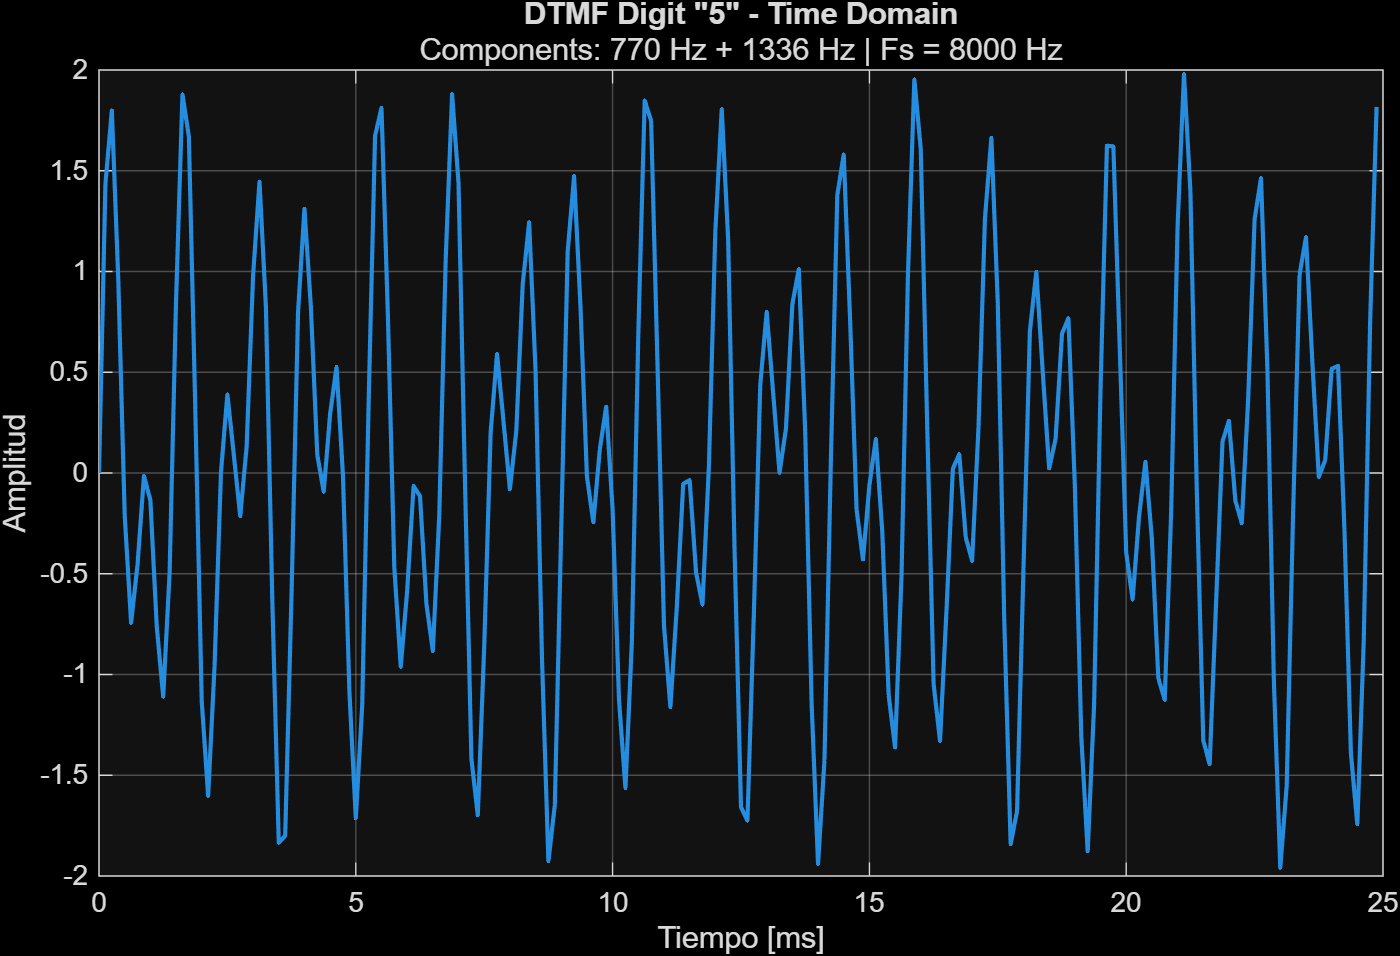
\includegraphics[width=\columnwidth]{images/01_tiempo_digito5.png}
\caption{Dominio del tiempo del dígito DTMF ``5'' (primeras 200 muestras), compuesto por la superposición de 770~Hz y 1336~Hz.}
\label{fig:tiempo_digito}
\end{figure}

\begin{figure}[!t]
\centering
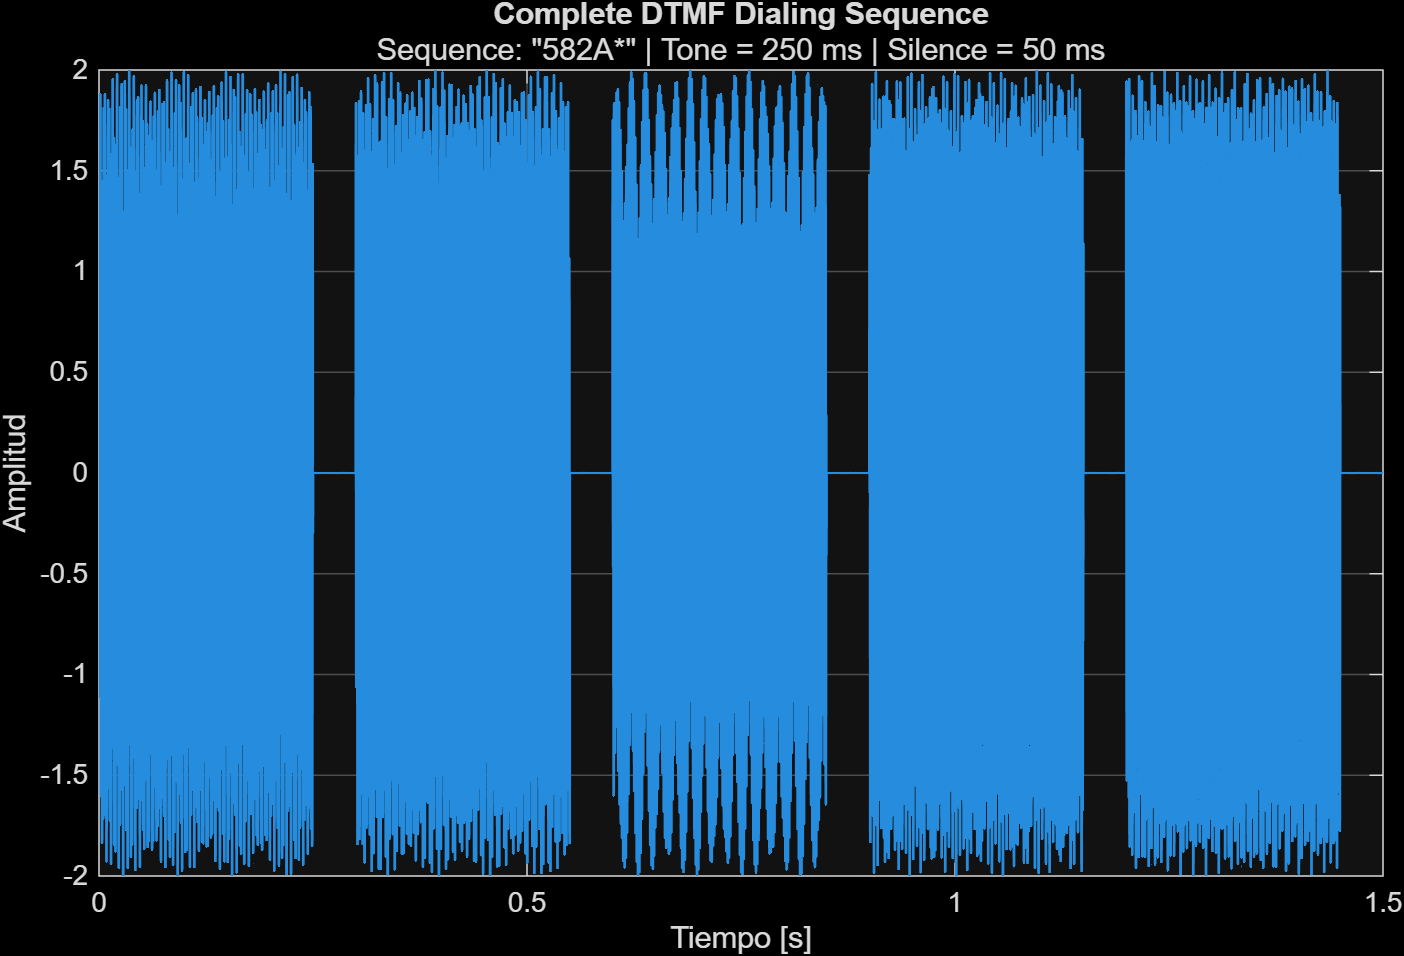
\includegraphics[width=\columnwidth]{images/02_tiempo_secuencia.png}
\caption{Secuencia completa de marcación DTMF ``582A*'', mostrando los cinco tonos separados por silencios de 50~ms.}
\label{fig:tiempo_secuencia}
\end{figure}

\subsection{Análisis espectral (FFT)}

La Figura \ref{fig:fft_digito} muestra el espectro de magnitud del dígito ``5'', donde se identifican dos picos dominantes cercanos a las frecuencias teóricas de 770~Hz y 1336~Hz. La Tabla \ref{tab:fft_resultados} resume la comparación entre las frecuencias teóricas y las detectadas mediante \texttt{findpeaks}, con una resolución espectral de la FFT de $\Delta f = F_s/N = 8000/2000 = 4$~Hz.

\begin{figure}[!t]
\centering
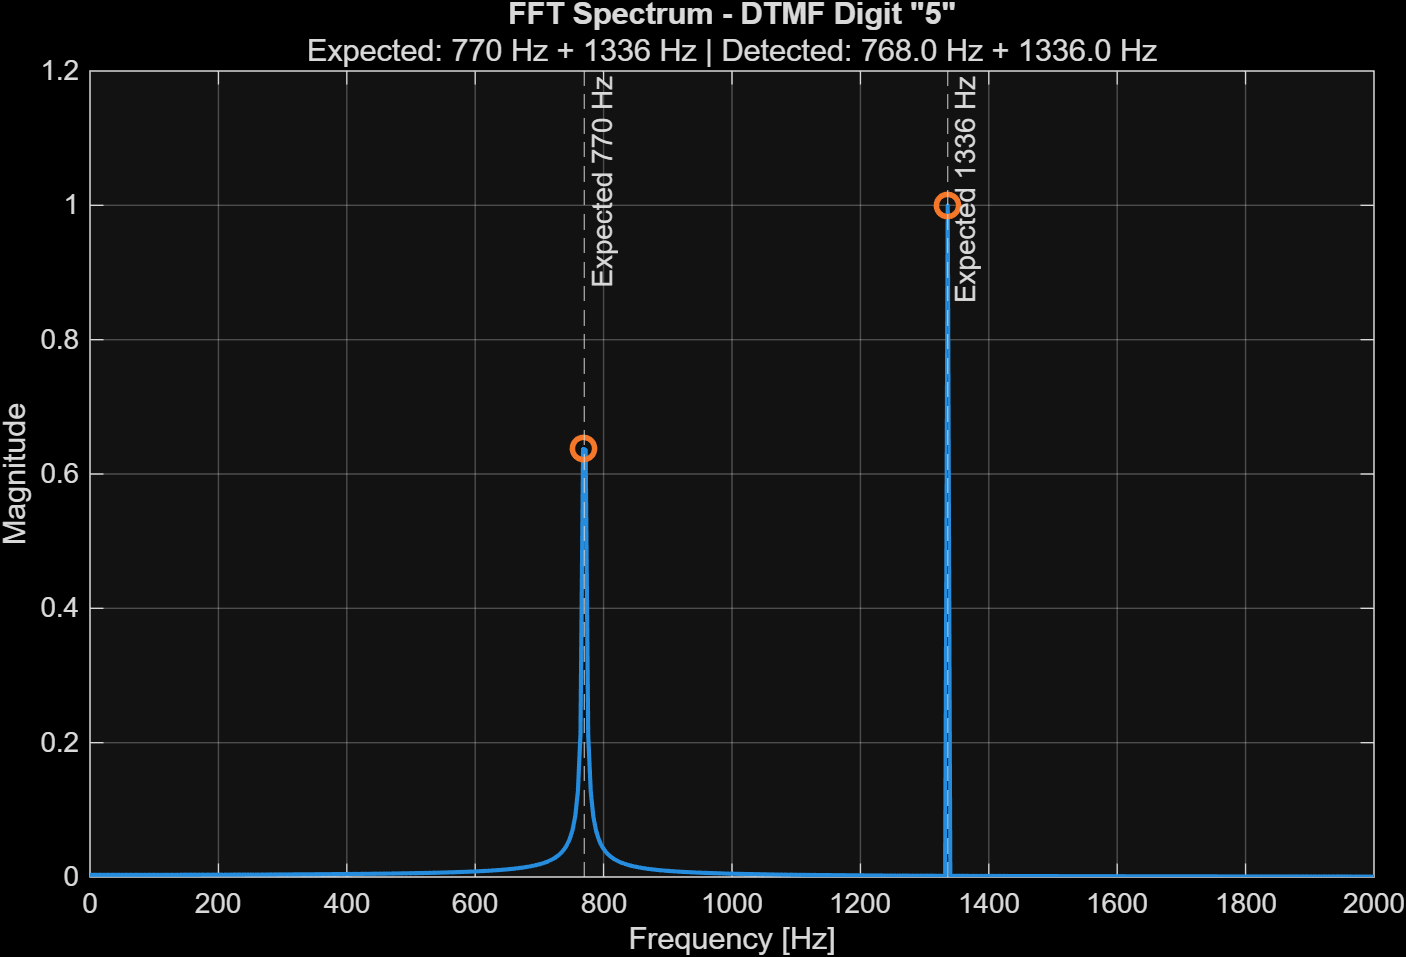
\includegraphics[width=\columnwidth]{images/03_fft_digito5.png}
\caption{Espectro FFT del dígito DTMF ``5'' con las frecuencias esperadas y detectadas señaladas.}
\label{fig:fft_digito}
\end{figure}

\begin{table}[!t]
\centering
\caption{Comparación entre frecuencias teóricas y detectadas para el dígito ``5''}
\label{tab:fft_resultados}
\begin{tabular}{|l|c|c|c|}
\hline
\textbf{Componente} & \textbf{Teórica (Hz)} & \textbf{Detectada (Hz)} & \textbf{Error (\%)} \\ \hline
Baja ($f_L$) & 770 & 768.0 & 0.260 \\ \hline
Alta ($f_H$) & 1336 & 1336.0 & 0.000 \\ \hline
\end{tabular}
\end{table}

El error de la componente baja (0.260\%) se explica por la resolución finita de la FFT ($\Delta f = 4$~Hz): al no existir necesariamente un contenedor (\textit{bin}) de frecuencia exactamente en 770~Hz, el pico detectado cae en el contenedor discreto más cercano (768~Hz), a solo 2~Hz del valor teórico, dentro de la resolución esperada.

\subsection{Comparación teórica vs. simulada y efecto del ruido AWGN}

La Figura \ref{fig:awgn} presenta el espectro del dígito ``5'' tras la adición de ruido AWGN para SNR de 30, 20, 10 y 0~dB.

\begin{figure}[!t]
\centering
\begin{minipage}{0.49\columnwidth}
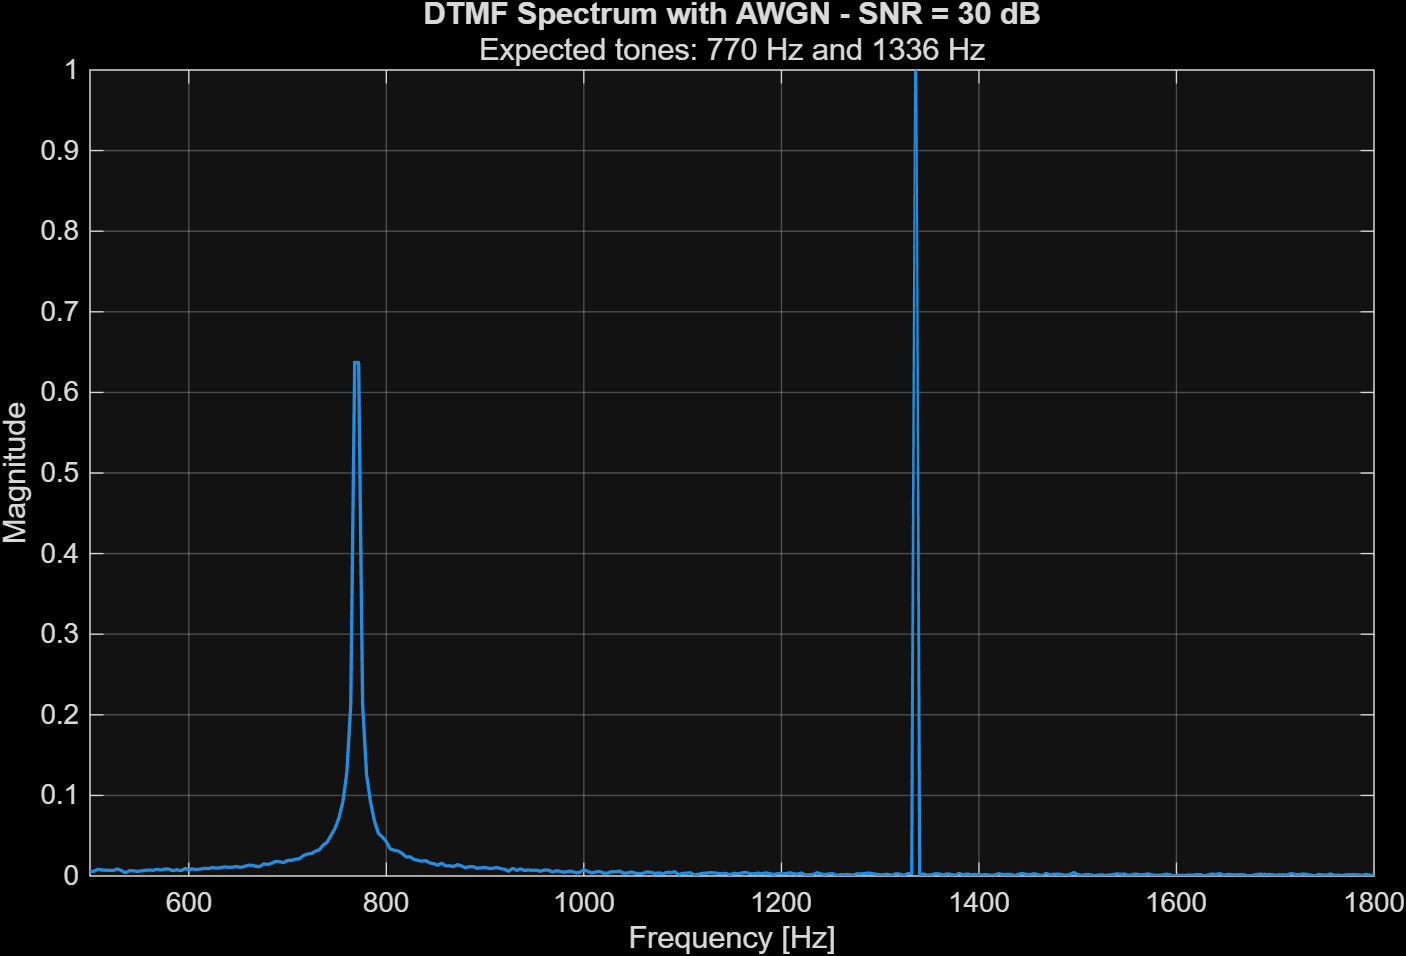
\includegraphics[width=\linewidth]{images/04_awgn_30db.png}
\end{minipage}\hfill
\begin{minipage}{0.49\columnwidth}
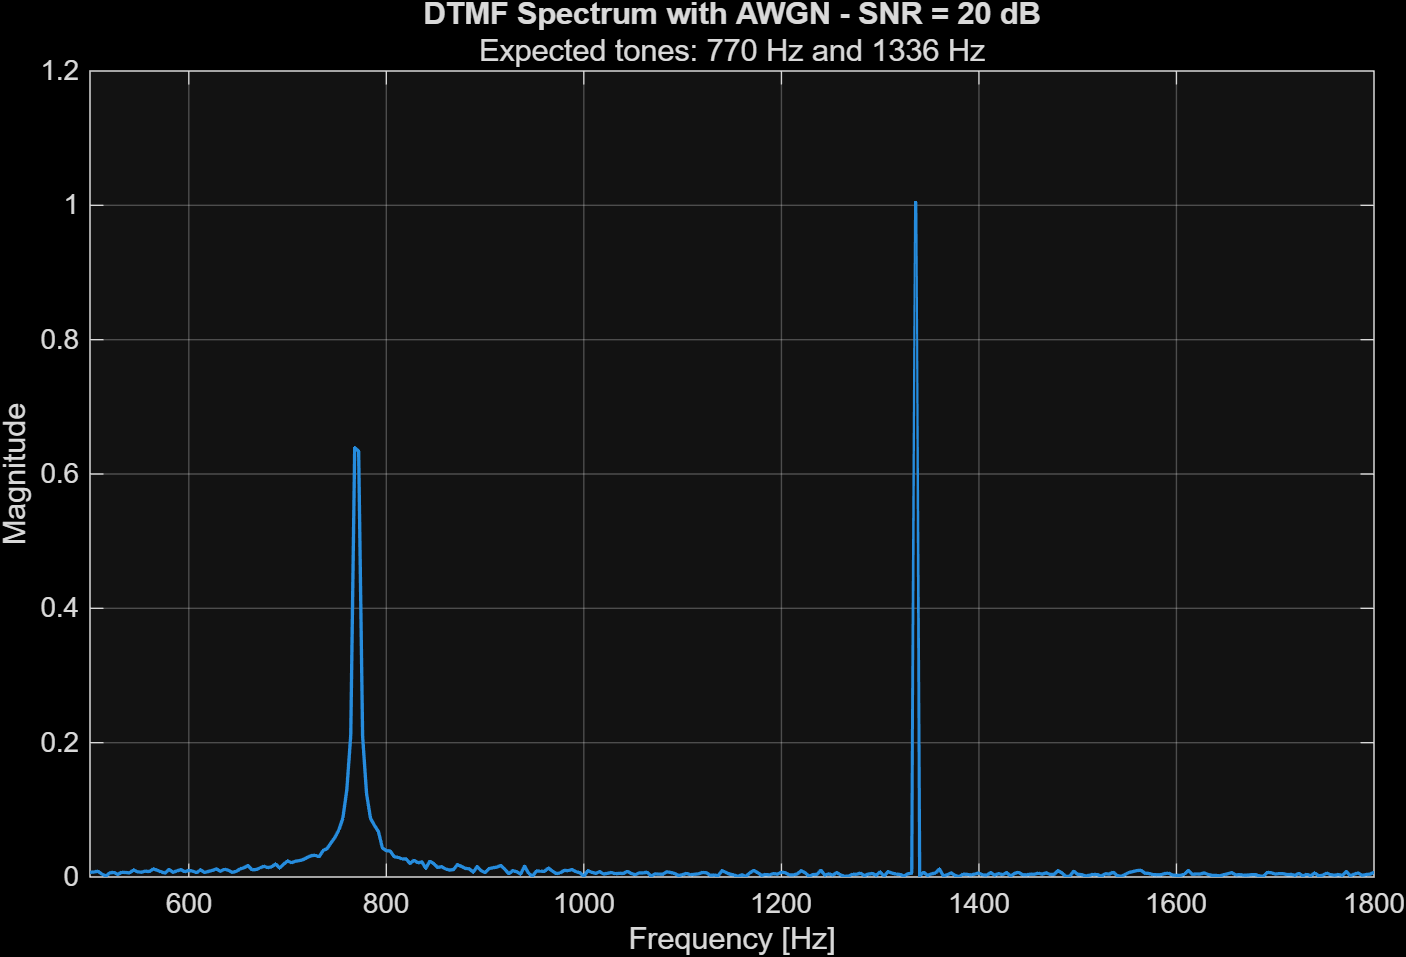
\includegraphics[width=\linewidth]{images/04_awgn_20db.png}
\end{minipage}

\vspace{0.3em}
\begin{minipage}{0.49\columnwidth}
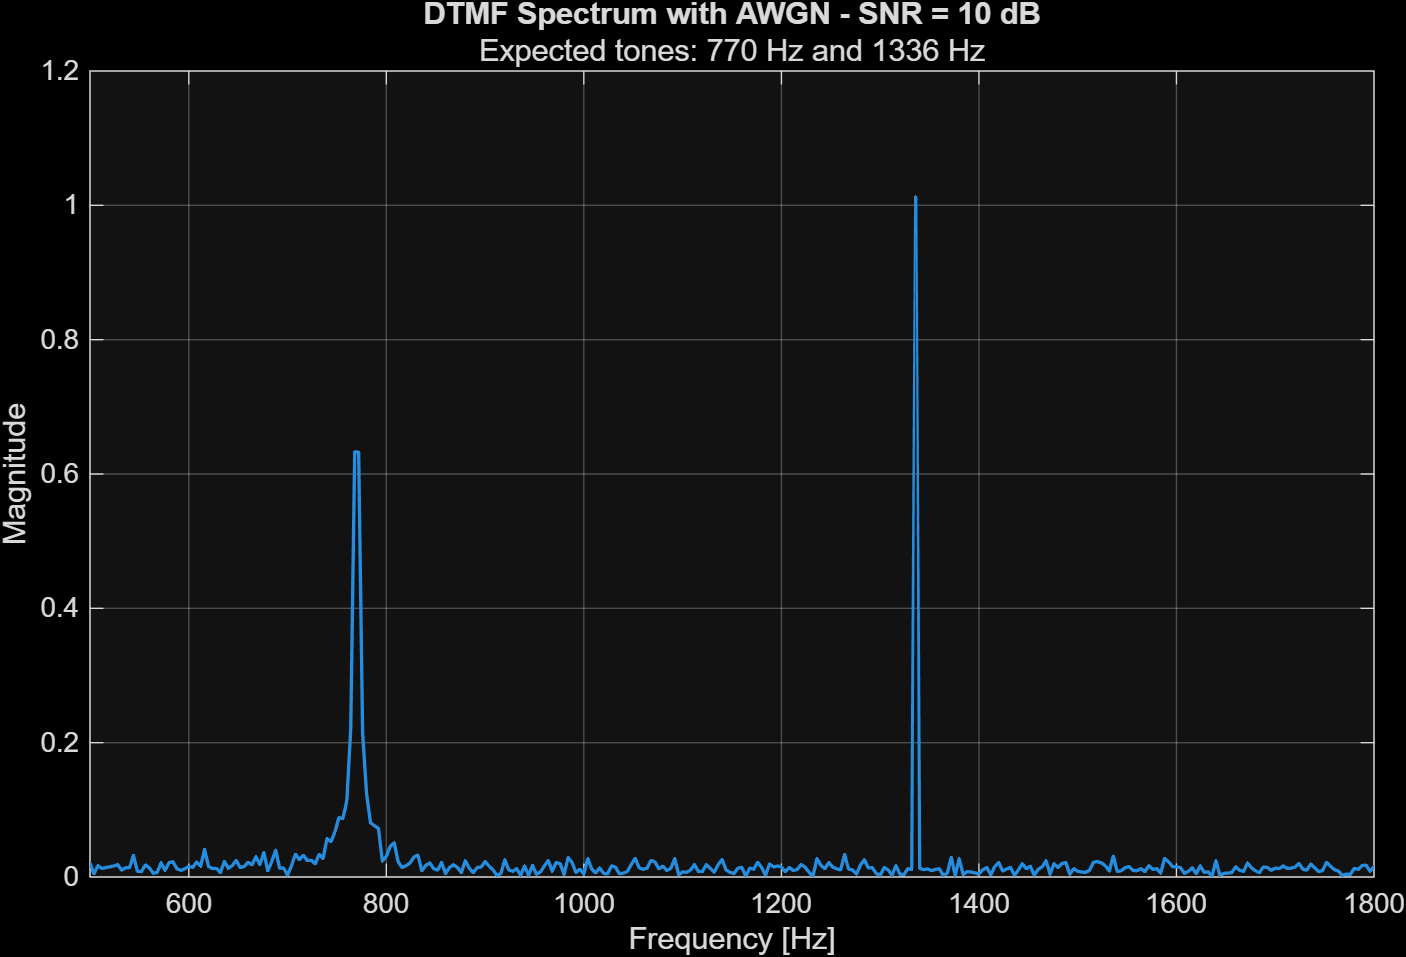
\includegraphics[width=\linewidth]{images/04_awgn_10db.png}
\end{minipage}\hfill
\begin{minipage}{0.49\columnwidth}
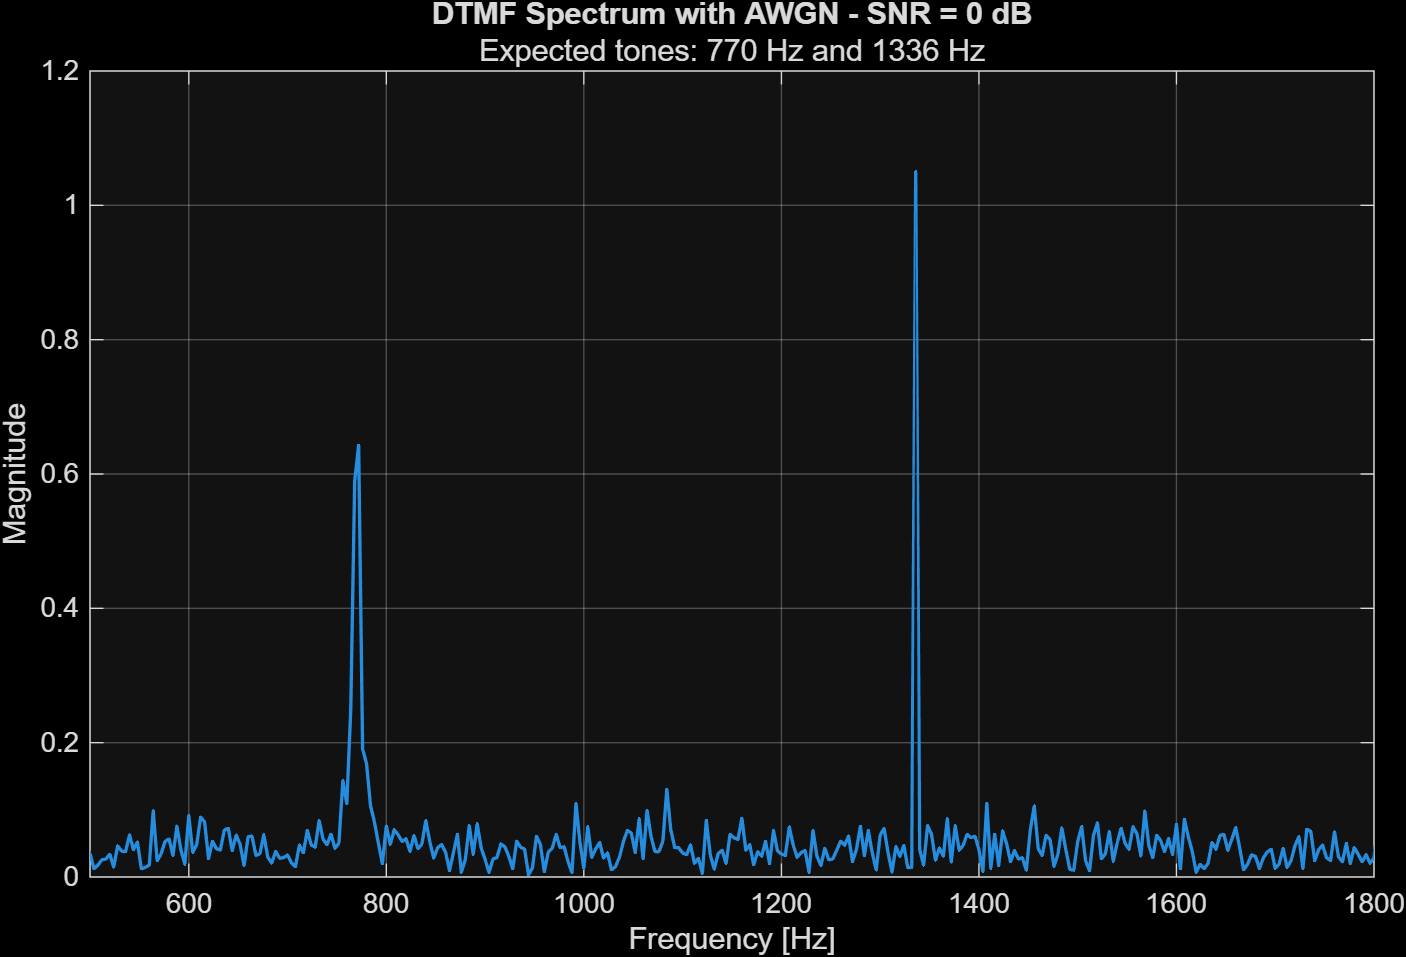
\includegraphics[width=\linewidth]{images/04_awgn_0db.png}
\end{minipage}
\caption{Espectro del dígito ``5'' con ruido AWGN para SNR de 30, 20, 10 y 0~dB (de izquierda a derecha, arriba a abajo).}
\label{fig:awgn}
\end{figure}

Para SNR de 30 y 20~dB, los dos picos DTMF se distinguen con claridad sobre un piso de ruido bajo. En 10~dB el piso de ruido se eleva de forma apreciable, aunque ambos picos siguen siendo identificables por encima de él. En 0~dB, la potencia del ruido iguala a la de la señal y el piso espectral se eleva hasta magnitudes comparables a las de los picos DTMF, dificultando severamente su discriminación visual y aumentando el riesgo de falsos picos.

\begin{itemize}
    \item \textbf{¿A partir de qué SNR se vuelve difícil identificar las dos frecuencias?} A partir de 0~dB la identificación se vuelve difícil, ya que el piso de ruido alcanza una magnitud comparable a la de los picos DTMF; en 10~dB los picos aún se distinguen con un margen razonable.
    \item \textbf{¿Cuál frecuencia (alta o baja) es más sensible al ruido?} Dado que el AWGN es blanco (densidad espectral de potencia constante en frecuencia) y ambos tonos comparten la misma amplitud, ambas componentes se ven afectadas de forma similar en términos de SNR local; sin embargo, en la práctica la componente de mayor frecuencia (1336~Hz) suele ser ligeramente más vulnerable en sistemas reales debido a la atenuación de alta frecuencia introducida por filtros de línea, lo cual no se modela en este AWGN puro pero es relevante para el diseño de detectores.
    \item \textbf{¿Se podría seguir detectando el dígito solo con FFT?} A 10~dB sí, empleando un criterio de altura mínima de pico adecuado. A 0~dB la FFT simple se vuelve poco confiable y sería necesario promediar múltiples ventanas o aplicar técnicas de filtrado previo (por ejemplo, banco de filtros pasa-banda centrados en las frecuencias DTMF) para recuperar una detección robusta.
\end{itemize}

\subsection{Duración del tono y resolución espectral}

La Figura \ref{fig:duracion} muestra el espectro del tono 770~Hz + 1336~Hz para duraciones de 50, 100, 250 y 500~ms. La Tabla \ref{tab:resolucion} resume la resolución espectral teórica $\Delta f = 1/T$ para cada duración.

\begin{table}[!t]
\centering
\caption{Resolución espectral teórica según la duración del tono}
\label{tab:resolucion}
\begin{tabular}{|c|c|}
\hline
\textbf{Duración $T$ (ms)} & \textbf{$\Delta f = 1/T$ (Hz)} \\ \hline
50 & 20 \\ \hline
100 & 10 \\ \hline
250 & 4 \\ \hline
500 & 2 \\ \hline
\end{tabular}
\end{table}

\begin{figure}[!t]
\centering
\begin{minipage}{0.49\columnwidth}
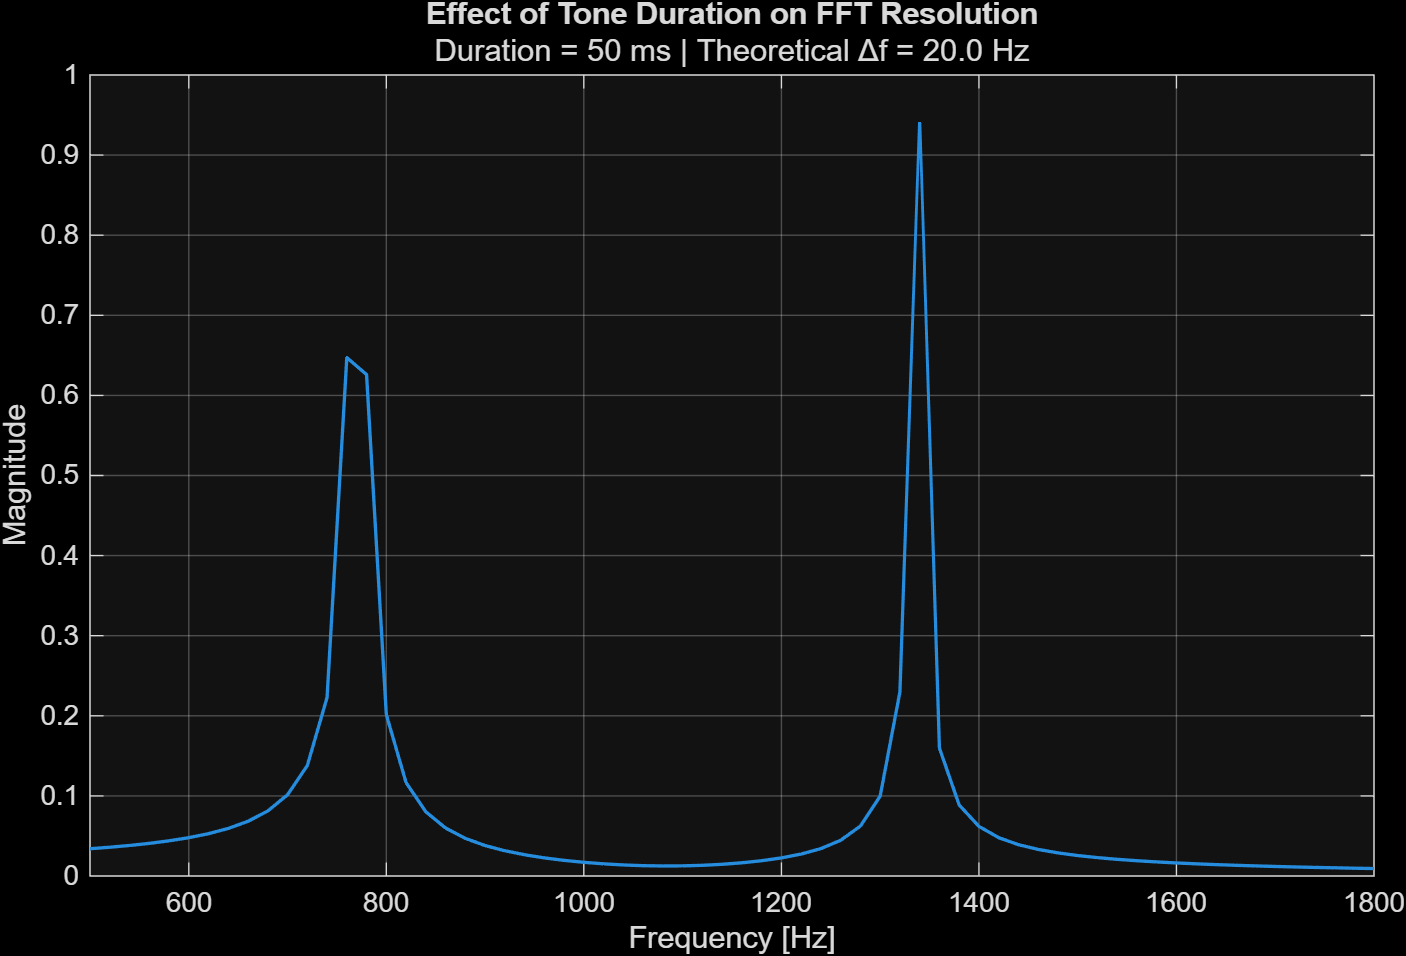
\includegraphics[width=\linewidth]{images/05_duracion_50ms.png}
\end{minipage}\hfill
\begin{minipage}{0.49\columnwidth}
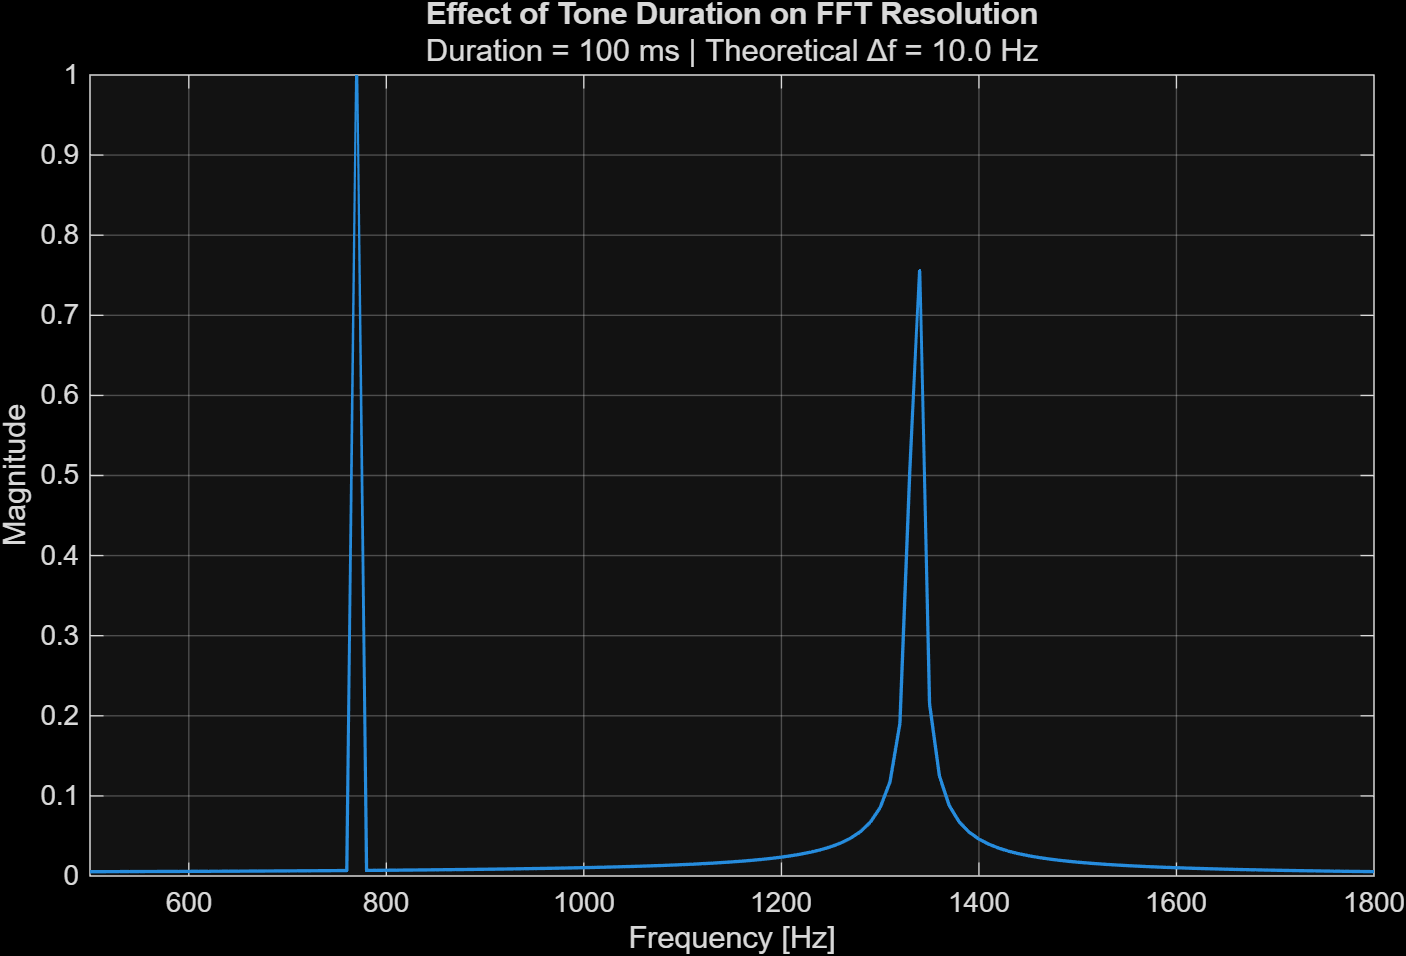
\includegraphics[width=\linewidth]{images/05_duracion_100ms.png}
\end{minipage}

\vspace{0.3em}
\begin{minipage}{0.49\columnwidth}
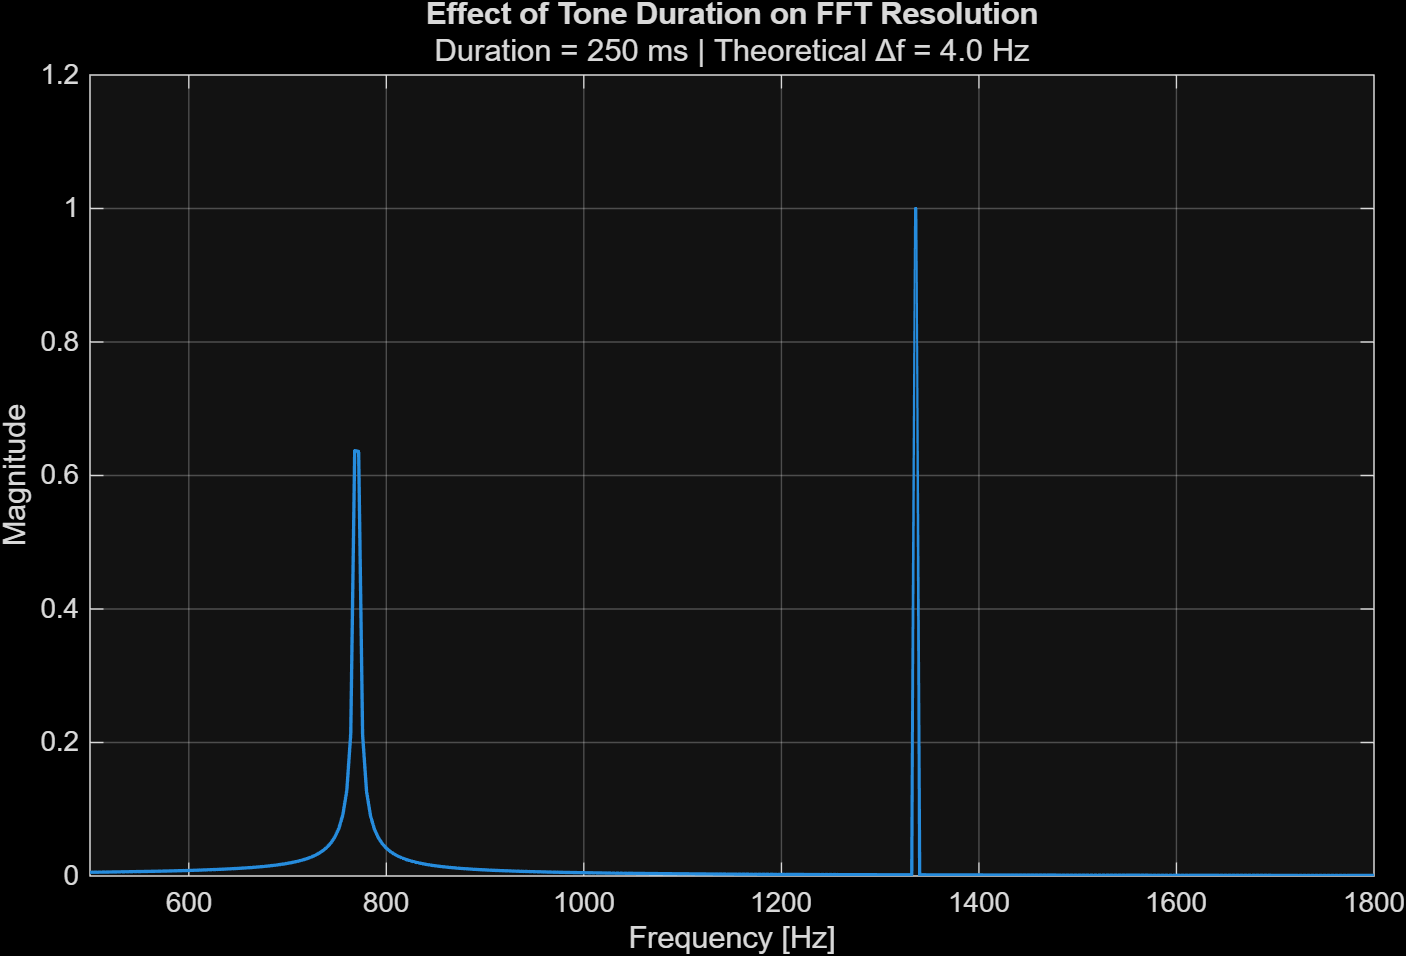
\includegraphics[width=\linewidth]{images/05_duracion_250ms.png}
\end{minipage}\hfill
\begin{minipage}{0.49\columnwidth}
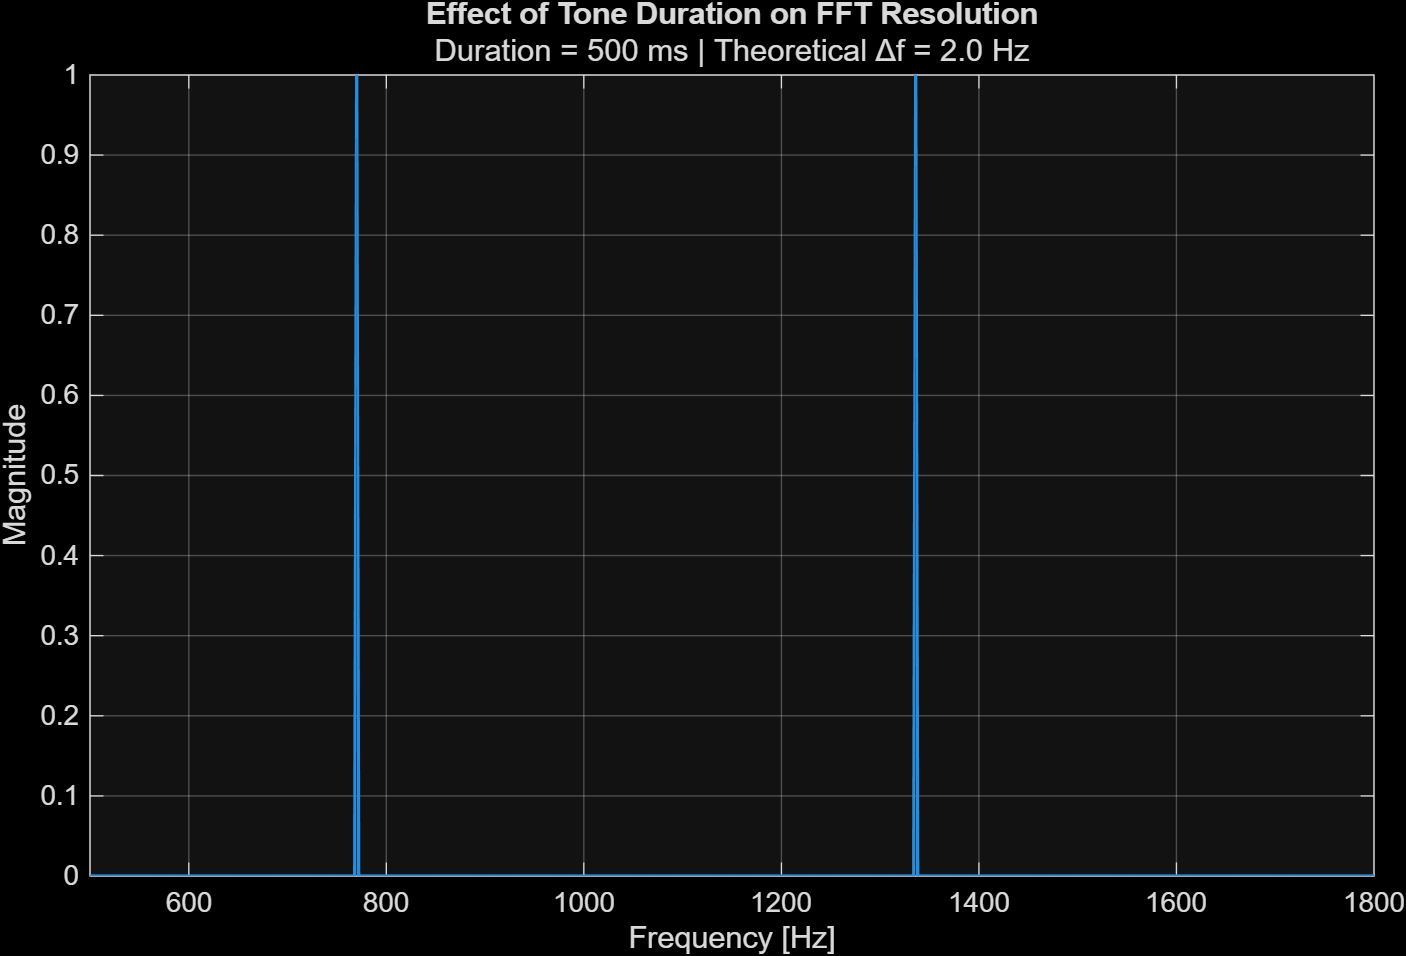
\includegraphics[width=\linewidth]{images/05_duracion_500ms.png}
\end{minipage}
\caption{Espectro del tono DTMF para duraciones de 50, 100, 250 y 500~ms (de izquierda a derecha, arriba a abajo). Los picos se estrechan al aumentar la duración.}
\label{fig:duracion}
\end{figure}

Se observa que, al aumentar la duración del tono, los picos espectrales se estrechan y las dos componentes (770~Hz y 1336~Hz) se separan con mayor claridad, en concordancia con la ecuación \eqref{eq:resolucion_espectral}. Con una duración de 50~ms, la resolución teórica es de apenas 20~Hz, generando picos anchos que, aunque en este caso las frecuencias DTMF están suficientemente separadas para distinguirse, reducen el margen de tolerancia frente a corrimientos por ruido o interferencia; en el límite, con tonos DTMF de dígitos con separación menor entre sí, una resolución tan gruesa podría provocar la fusión aparente de picos o una localización imprecisa del máximo. Duraciones cortas de tono, por lo tanto, dificultan la detección DTMF porque reducen el número de ciclos completos observados de cada componente, ensanchando su lóbulo principal en el espectro y disminuyendo la relación entre la altura del pico y el piso de fuga espectral (\textit{spectral leakage}).

\subsection{Atenuación de línea telefónica}

La Figura \ref{fig:atenuacion} muestra la señal en el dominio del tiempo del dígito ``5'' para atenuaciones de 0, $-6$, $-12$ y $-20$~dB, calculadas mediante la ecuación \eqref{eq:atenuacion} (factores lineales de 1.000, 0.501, 0.251 y 0.100, respectivamente).

\begin{figure}[!t]
\centering
\begin{minipage}{0.49\columnwidth}
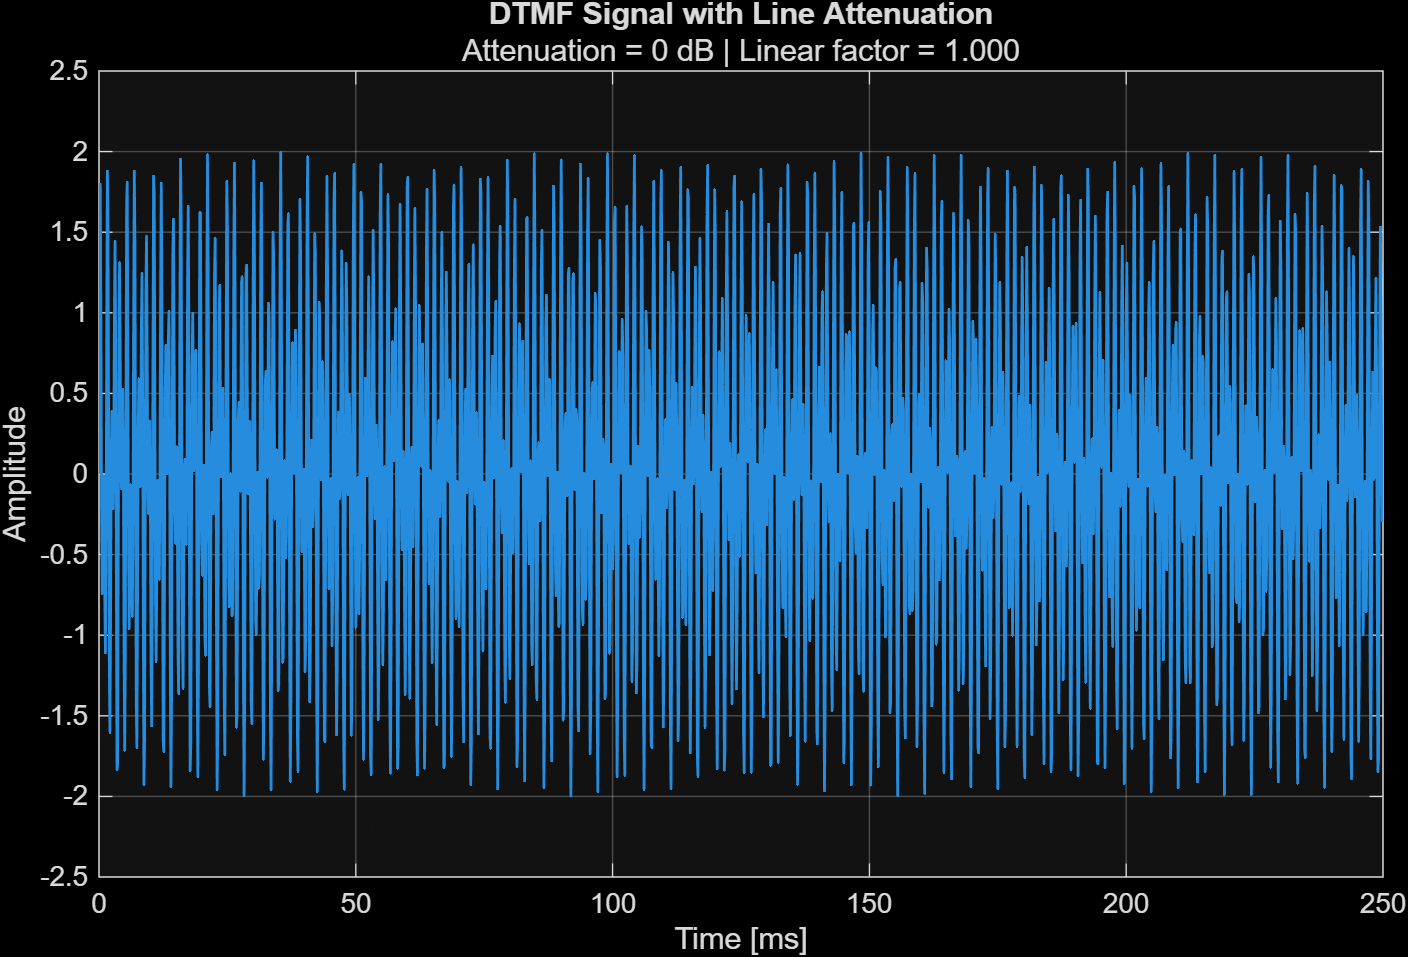
\includegraphics[width=\linewidth]{images/06_atenuacion_0db.png}
\end{minipage}\hfill
\begin{minipage}{0.49\columnwidth}
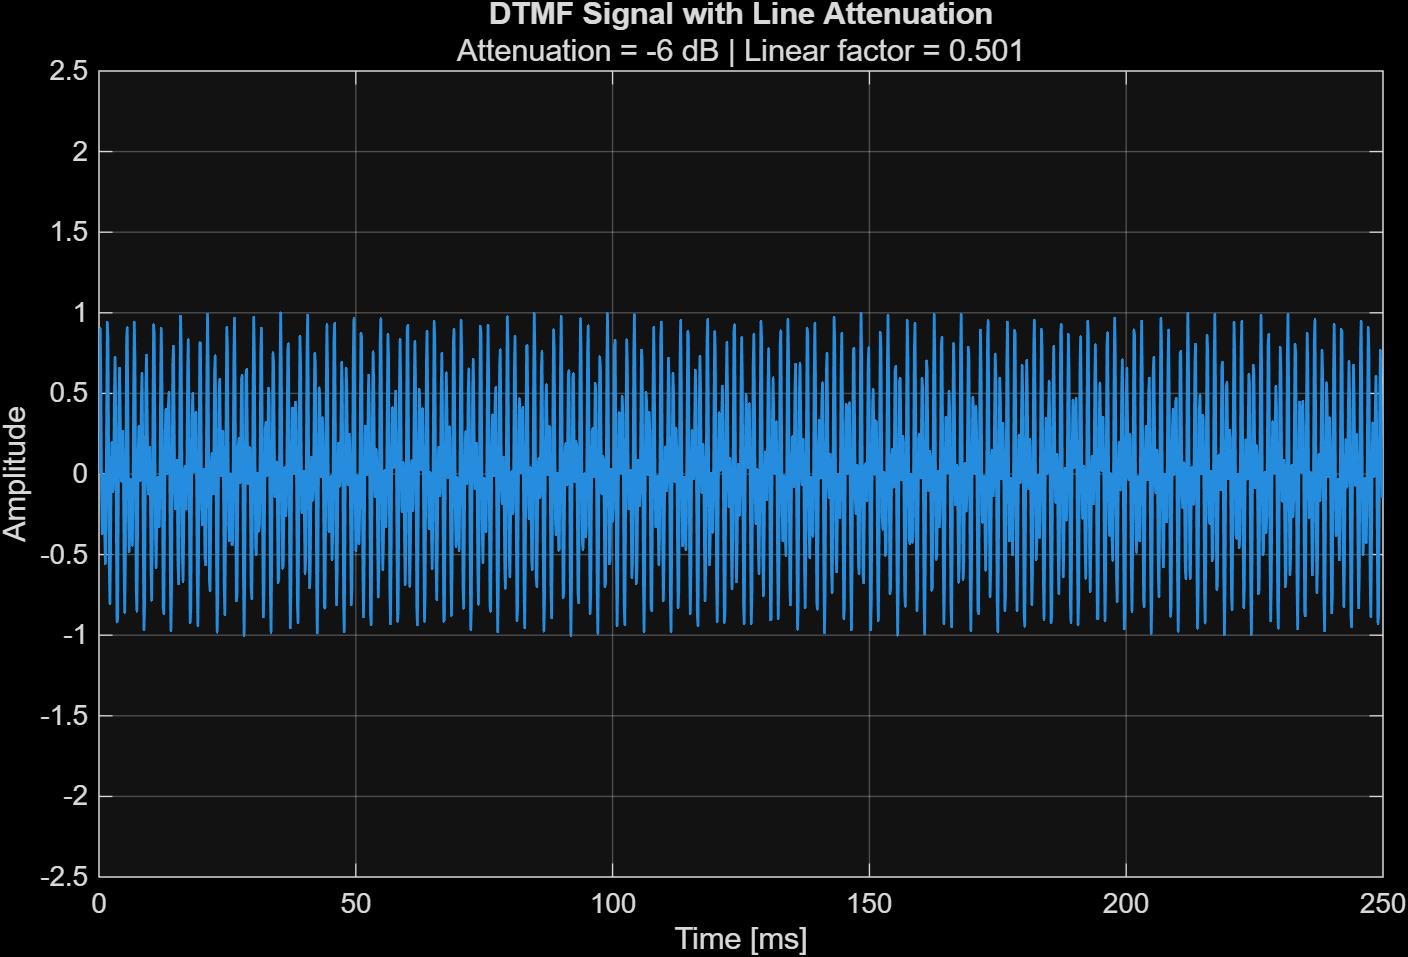
\includegraphics[width=\linewidth]{images/06_atenuacion_-6db.png}
\end{minipage}

\vspace{0.3em}
\begin{minipage}{0.49\columnwidth}
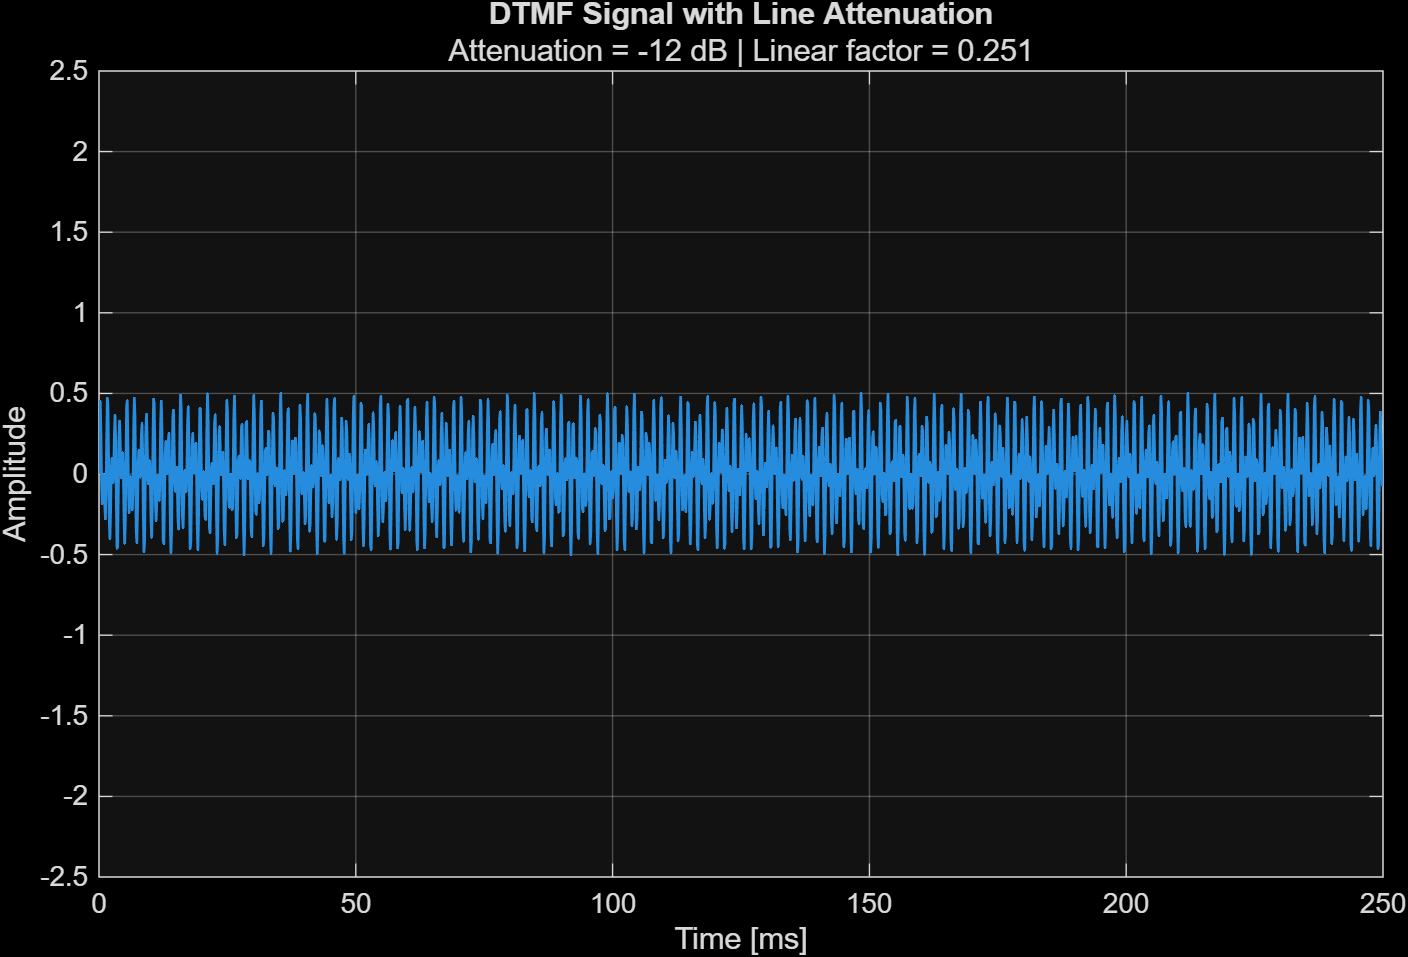
\includegraphics[width=\linewidth]{images/06_atenuacion_-12db.png}
\end{minipage}\hfill
\begin{minipage}{0.49\columnwidth}
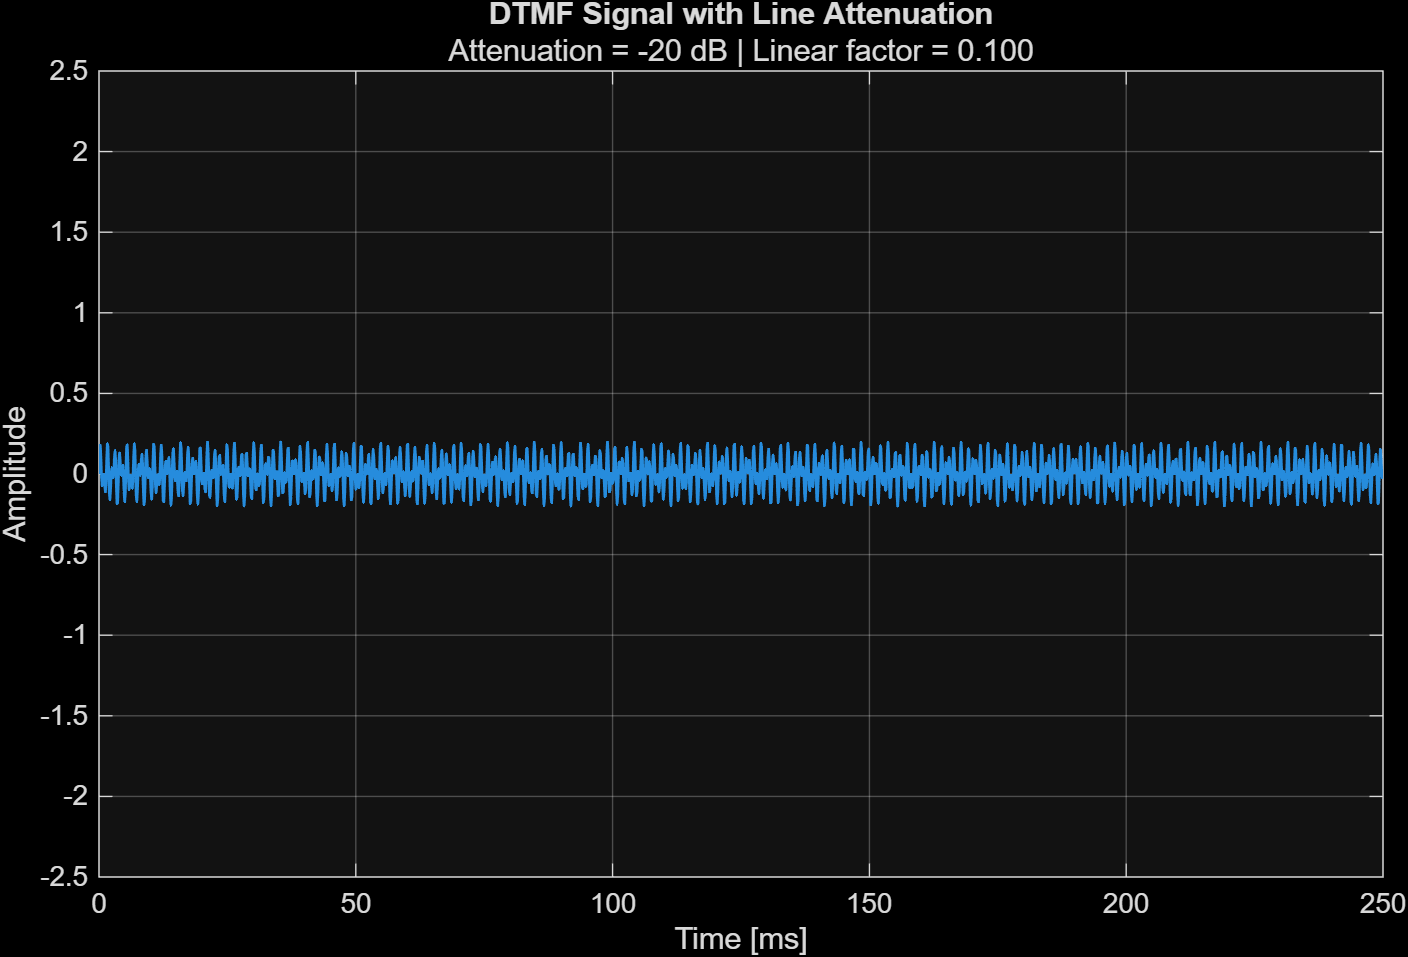
\includegraphics[width=\linewidth]{images/06_atenuacion_-20db.png}
\end{minipage}
\caption{Señal DTMF en el dominio del tiempo para atenuaciones de línea de 0, $-6$, $-12$ y $-20$~dB (de izquierda a derecha, arriba a abajo).}
\label{fig:atenuacion}
\end{figure}

Como se aprecia en la Figura \ref{fig:atenuacion}, la amplitud pico de la señal se reduce proporcionalmente al factor lineal de atenuación, mientras que la forma de onda y, por extensión, el contenido frecuencial permanecen invariables: la atenuación es un escalamiento puramente multiplicativo en el dominio del tiempo, por lo que en el dominio de la frecuencia solo reduce la magnitud del espectro sin desplazar la posición de los picos. Un detector basado únicamente en la posición de los picos espectrales no debería fallar por atenuación pura; sin embargo, un detector que dependa de un umbral fijo de magnitud (\textit{threshold}) sí podría fallar si la atenuación reduce la amplitud del pico por debajo de dicho umbral, o si la atenuación reduce el margen efectivo de SNR frente al ruido del canal real. Este efecto es representativo de líneas telefónicas largas o deterioradas, donde la resistencia distribuida del cableado y las pérdidas de acoplamiento atenúan la señal antes de llegar a la central, exigiendo receptores con ganancia automática (AGC) o umbrales de detección adaptativos.

\subsection{Decodificador automático}

La Tabla \ref{tab:decoder} resume los resultados del decodificador automático aplicado a la secuencia completa ``582A*''. Los cinco dígitos fueron identificados correctamente, validando el algoritmo de segmentación, FFT por bloques y búsqueda de picos en el rango 600--1700~Hz descrito en la Sección IV-G.

\begin{table}[!t]
\centering
\caption{Resultados del decodificador automático para la secuencia ``582A*''}
\label{tab:decoder}
\begin{tabular}{|c|c|c|c|c|c|}
\hline
\textbf{Pos.} & \textbf{Esp.} & \textbf{Detec.} & \textbf{$f_L$ (Hz)} & \textbf{$f_H$ (Hz)} & \textbf{Correcto} \\ \hline
1 & 5 & 5 & 768 & 1336 & Sí \\ \hline
2 & 8 & 8 & 852 & 1336 & Sí \\ \hline
3 & 2 & 2 & 696 & 1336 & Sí \\ \hline
4 & A & A & 696 & 1632 & Sí \\ \hline
5 & * & * & 940 & 1208 & Sí \\ \hline
\end{tabular}
\end{table}

El decodificador reconoció el 100\% de los dígitos de la secuencia (5/5), con desviaciones de hasta 2~Hz respecto a las frecuencias teóricas, consistentes con la resolución espectral de $\Delta f = 4$~Hz de la FFT de 2000 muestras utilizada.

\subsection{Simulación complementaria en Simulink}

El modelo \texttt{mi\_modelo\_dtmf} reproduce la generación y muestreo del tono 770~Hz + 1336~Hz mediante bloques funcionales. La Figura \ref{fig:simulink_tiempo} muestra un acercamiento a los primeros 30~ms de la señal muestreada, la Figura \ref{fig:simulink_tiempo_completo} la simulación completa de 0.25~s, y las Figuras \ref{fig:simulink_fft} y \ref{fig:simulink_fft_zoom} el espectro resultante en el rango completo (0--2000~Hz) y en un acercamiento (500--1600~Hz), respectivamente.

\begin{figure}[!t]
\centering
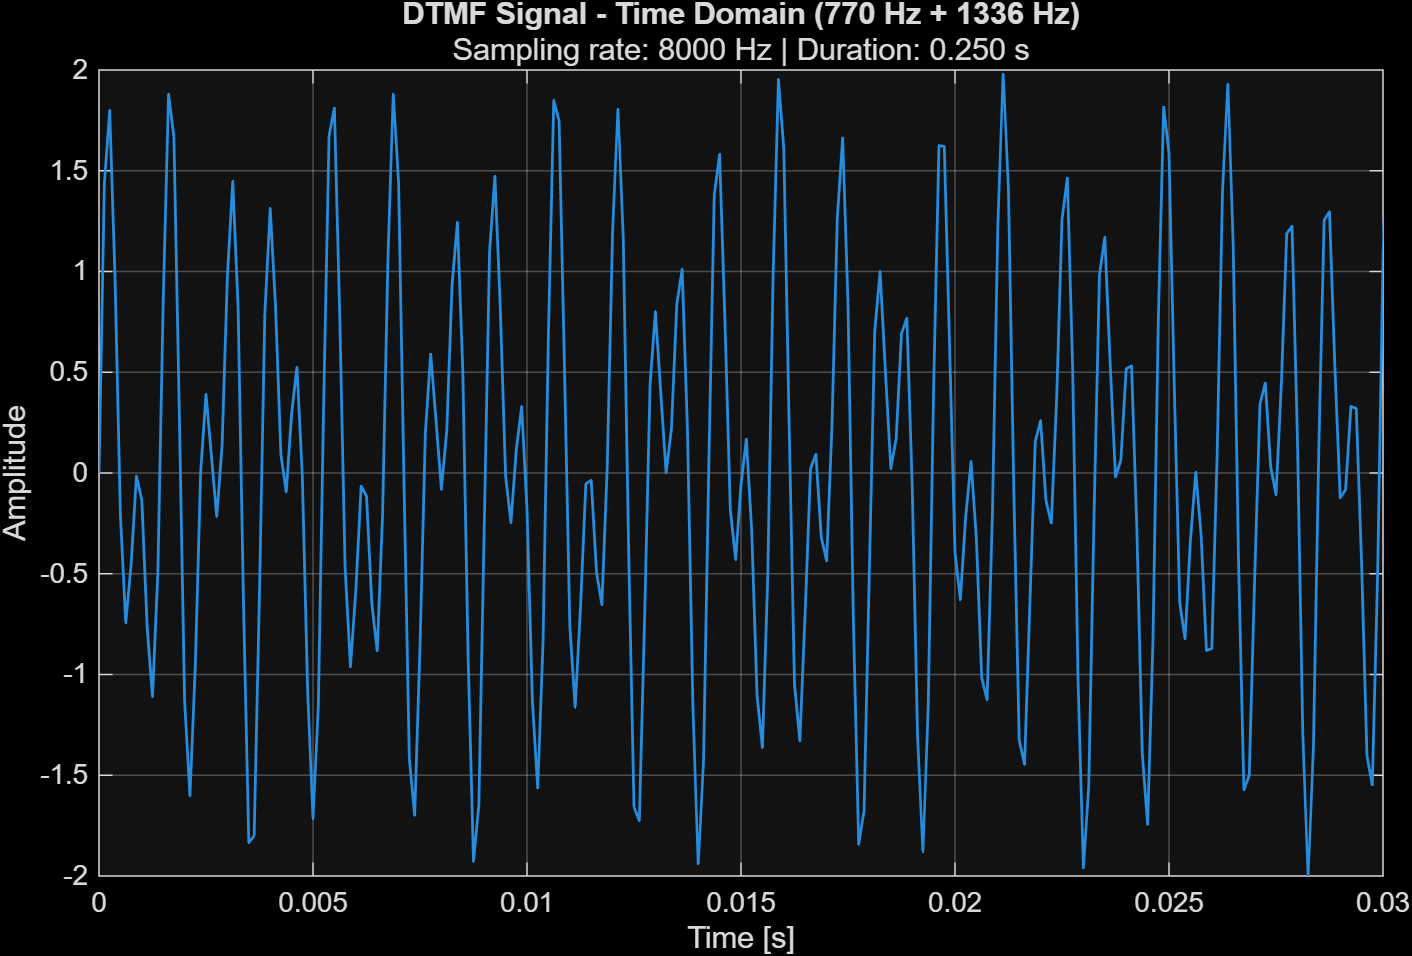
\includegraphics[width=\columnwidth]{images/07_simulink_tiempo_zoom.png}
\caption{Modelo Simulink: dominio del tiempo, acercamiento a los primeros 30~ms.}
\label{fig:simulink_tiempo}
\end{figure}

\begin{figure}[!t]
\centering
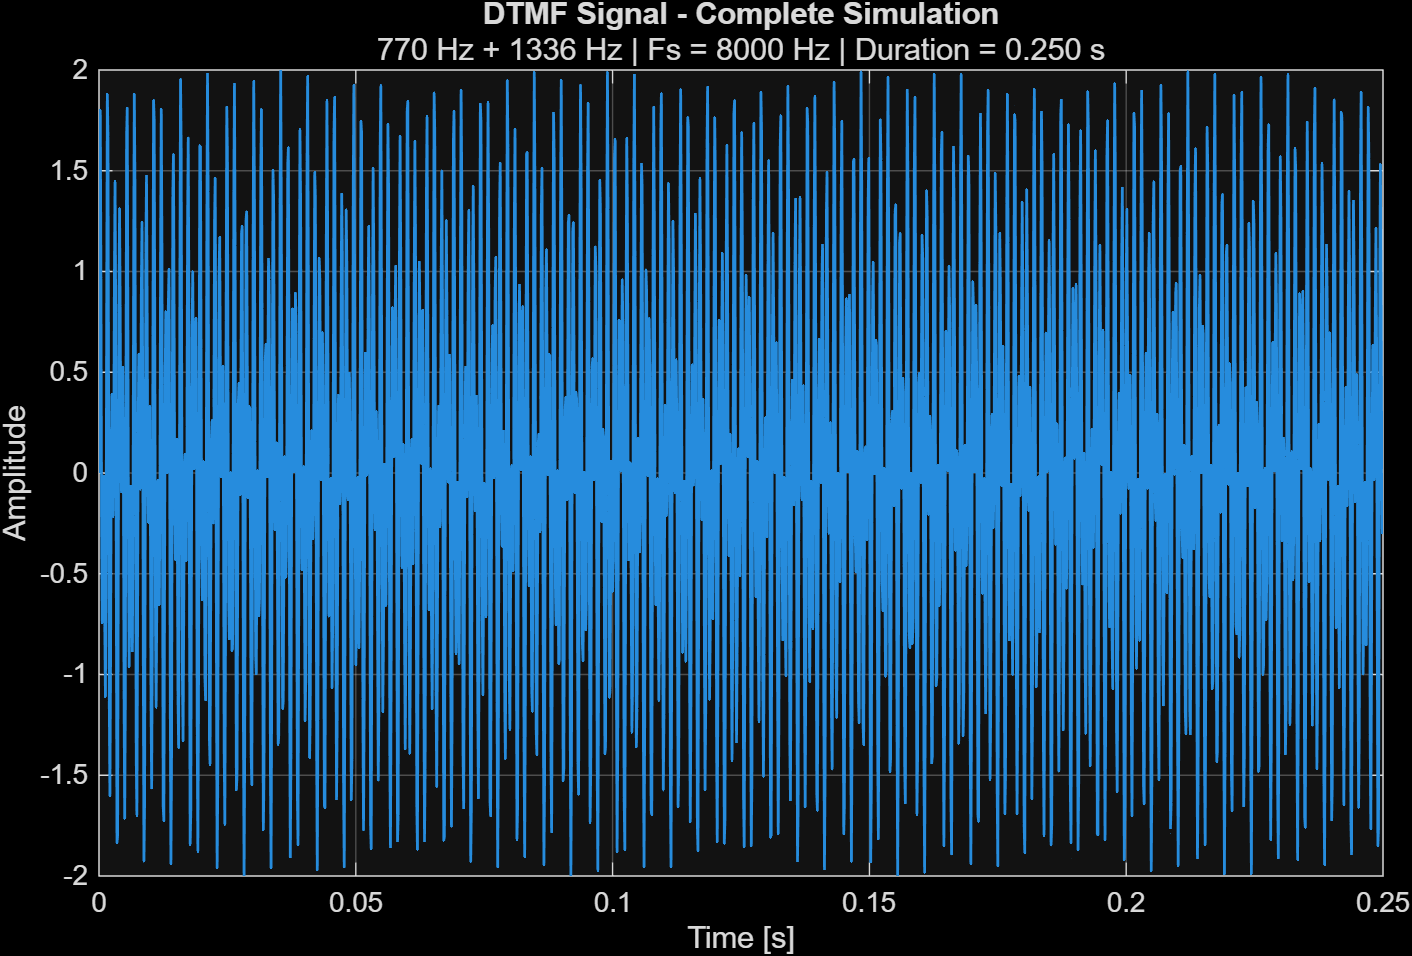
\includegraphics[width=\columnwidth]{images/08_simulink_tiempo_completo.png}
\caption{Modelo Simulink: señal completa muestreada durante 0.25~s.}
\label{fig:simulink_tiempo_completo}
\end{figure}

\begin{figure}[!t]
\centering
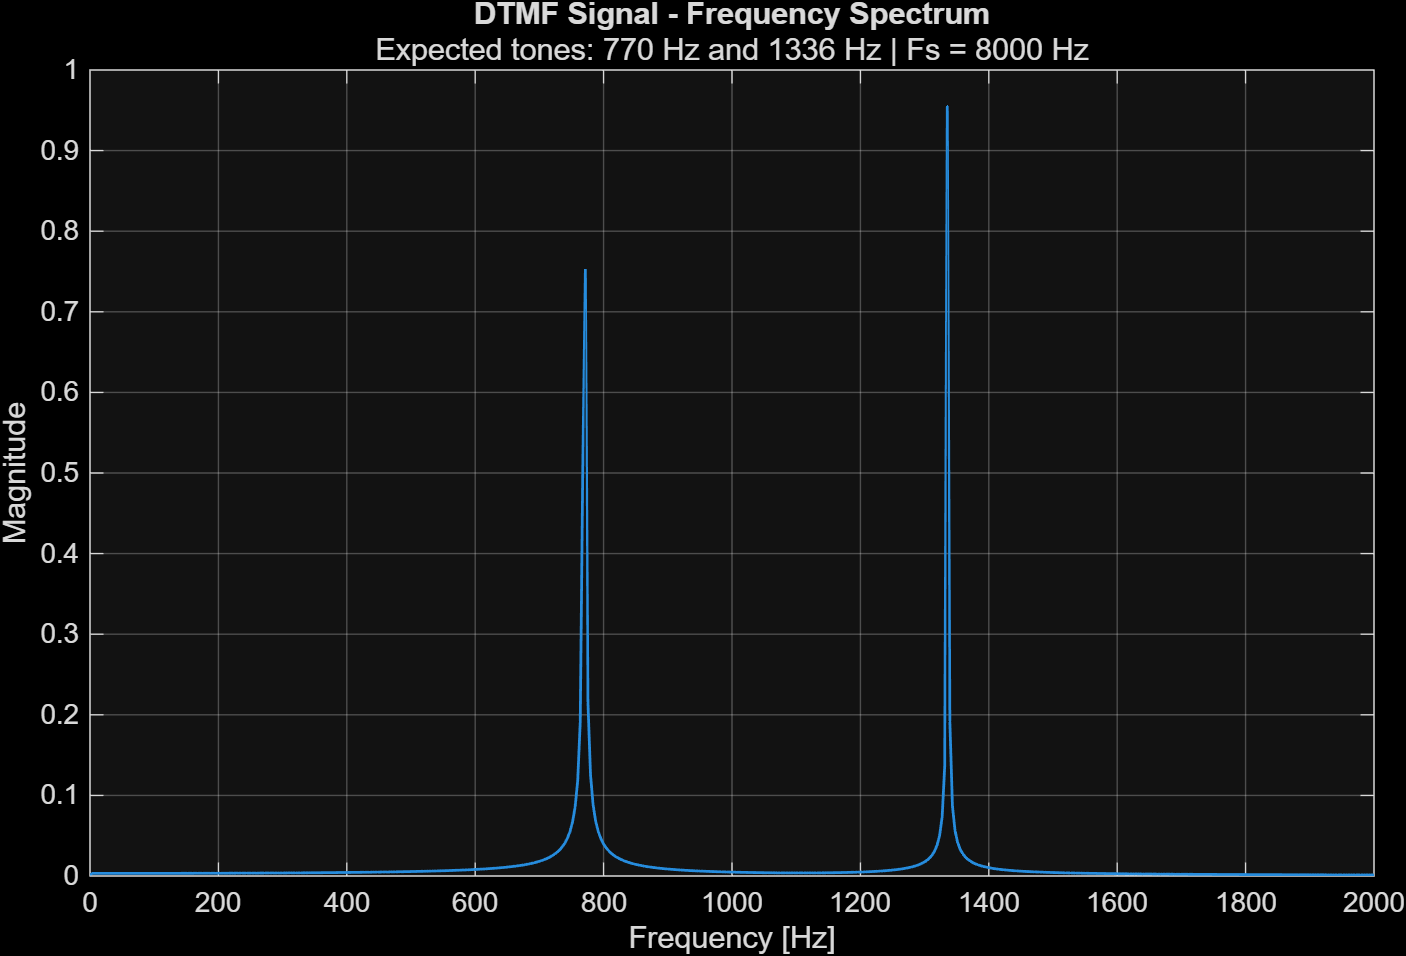
\includegraphics[width=\columnwidth]{images/09_simulink_fft_espectro.png}
\caption{Modelo Simulink: espectro FFT de la señal muestreada (0--2000~Hz).}
\label{fig:simulink_fft}
\end{figure}

\begin{figure}[!t]
\centering
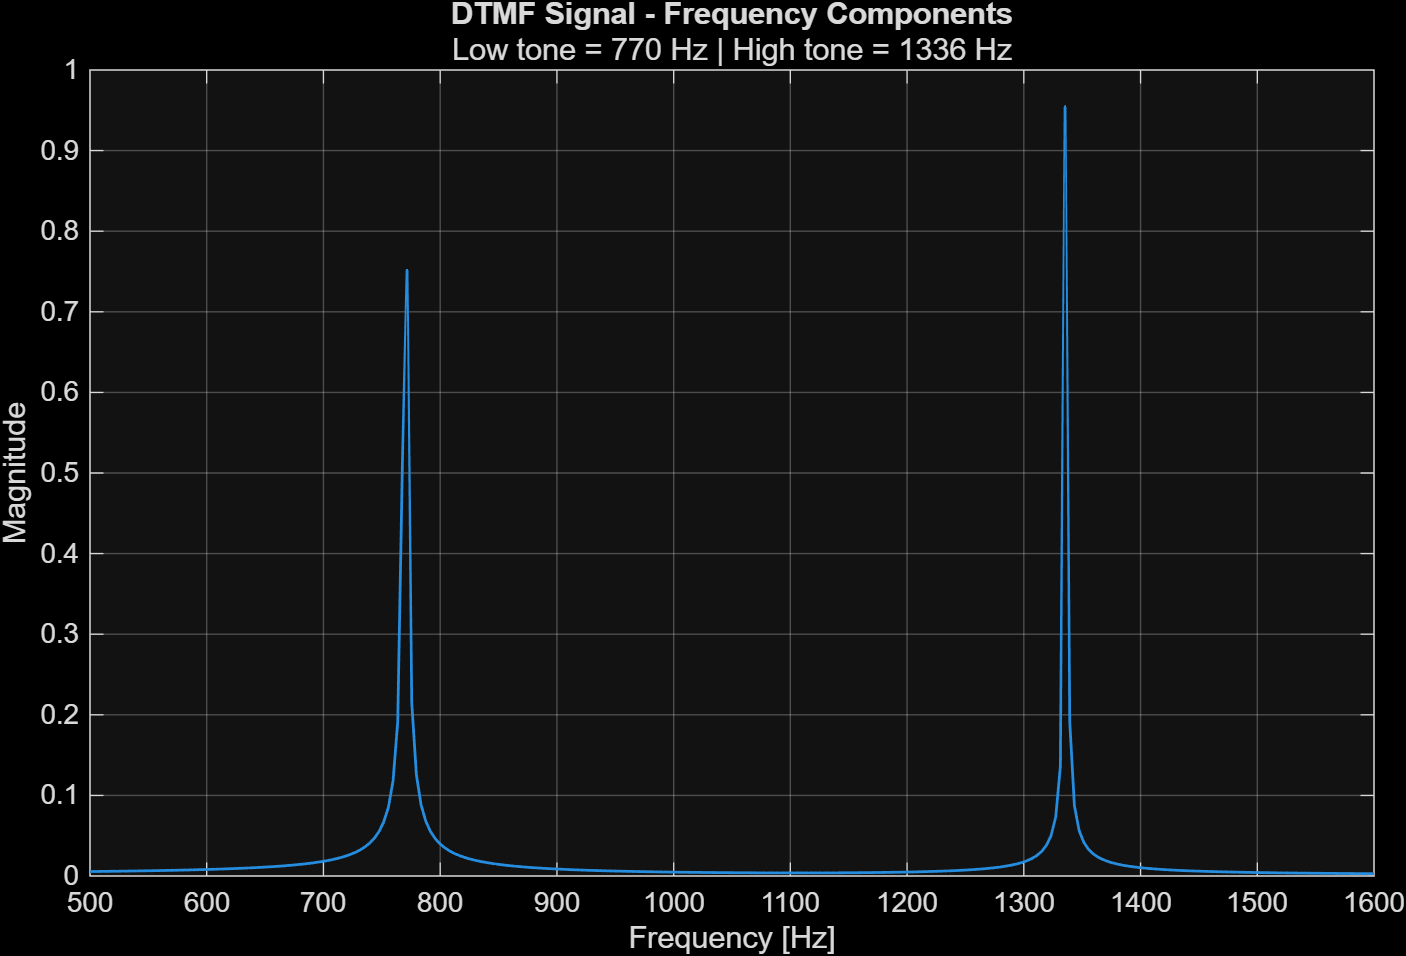
\includegraphics[width=\columnwidth]{images/10_simulink_fft_zoom.png}
\caption{Modelo Simulink: acercamiento del espectro FFT (500--1600~Hz) sobre las componentes DTMF.}
\label{fig:simulink_fft_zoom}
\end{figure}

La Tabla \ref{tab:simulink} compara las frecuencias teóricas con las detectadas a partir de la señal generada por el modelo Simulink.

\begin{table}[!t]
\centering
\caption{Resultados de detección de frecuencia del modelo Simulink}
\label{tab:simulink}
\begin{tabular}{|l|c|c|c|}
\hline
\textbf{Componente} & \textbf{Teórica (Hz)} & \textbf{Detectada (Hz)} & \textbf{Error (\%)} \\ \hline
Baja ($f_L$) & 770 & 771.61 & 0.210 \\ \hline
Alta ($f_H$) & 1336 & 1335.33 & 0.050 \\ \hline
\end{tabular}
\end{table}

Con una longitud de simulación de 0.25~s a $F_s = 8000$~Hz, la resolución espectral de la FFT resultó de 3.998~Hz, consistente con la obtenida en el script principal. Los errores porcentuales (0.210\% y 0.050\%) son del mismo orden de magnitud que los observados en la Sección V-B, confirmando que el modelo por bloques (fuente sinusoidal, suma, retenedor de orden cero y exportación a \textit{workspace}) reproduce fielmente la generación matemática directa de la señal DTMF.

\section{Discusión Integrada (Obligatoria)}

\textbf{¿Cuál condición afecta más la detección DTMF: ruido, duración o atenuación?} De las tres condiciones evaluadas, el ruido AWGN es la que más compromete la detección DTMF. Mientras que la atenuación de línea, dentro del rango evaluado (0 a $-20$~dB), solo reduce la amplitud del espectro sin desplazar los picos ni degradar la relación entre ellos y un piso de ruido nulo, y la reducción de duración del tono (hasta 50~ms) ensancha los picos sin llegar a impedir su identificación, el ruido AWGN eleva directamente el piso espectral hasta niveles comparables a los picos útiles cuando el SNR se aproxima a 0~dB, degradando la relación señal-piso de forma mucho más severa. En un sistema real, la atenuación de línea es relevante principalmente porque reduce el SNR efectivo al acercar la señal al piso de ruido térmico o de interferencia del canal, por lo que su efecto más peligroso es indirecto, a través de la interacción con el ruido, y no por sí sola.

\textbf{¿Por qué DTMF es robusto para telefonía?} DTMF es robusto porque cada dígito se codifica como la suma de dos tonos puros seleccionados de dos grupos de frecuencias disjuntos y sin relación armónica simple entre sí, lo que reduce drásticamente la probabilidad de que la voz humana, cuyo espectro es de banda ancha y variable en el tiempo, o el ruido de línea, generen falsamente un patrón de dos picos estables coincidentes con una combinación válida del teclado. Además, el uso de dos frecuencias simultáneas (en vez de una sola) añade redundancia: un detector requiere confirmar la presencia conjunta de ambas componentes antes de declarar un dígito válido, lo cual reduce la tasa de falsos positivos. La amplitud relativamente alta y estable de los tonos, generados electrónicamente en el propio equipo terminal, junto con duraciones mínimas normalizadas (típicamente no menores a 40--50~ms), garantiza además una resolución espectral suficiente para la separación de frecuencias vecinas de la tabla DTMF.

\textbf{¿Qué mejoras propondría para un detector real?} Se proponen las siguientes mejoras: (1) emplear el algoritmo de Goertzel en lugar de una FFT completa, evaluando únicamente las ocho frecuencias DTMF de interés, lo cual reduce el costo computacional y permite ventanas de análisis más cortas sin sacrificar precisión en las frecuencias relevantes; (2) incorporar un banco de filtros pasa-banda centrados en cada frecuencia DTMF antes de la etapa de detección, mejorando el SNR efectivo al eliminar energía fuera de banda; (3) implementar control automático de ganancia (AGC) para compensar la atenuación de línea antes de aplicar un umbral de detección fijo; (4) validar la duración mínima y la estabilidad temporal del tono detectado (\textit{debouncing}) para rechazar transitorios espurios; y (5) aplicar criterios de verificación de ``twist'' (relación de amplitud máxima permitida entre la componente alta y la baja) para descartar detecciones espurias generadas por voz o música.

\section{Consideraciones Conceptuales: LabVIEW y Simulink}

Esta sección responde a los ejercicios de LabVIEW realizados en el laboratorio (con evidencia gráfica propia) y, de forma conceptual, a las preguntas de análisis sobre el modelo Simulink \texttt{dspdtmf} planteadas en la guía. No se ejecutó el modelo de referencia \texttt{dspdtmf} de MathWorks en este trabajo, por lo que la discusión sobre dicho modelo se presenta sin figuras asociadas, complementaria a los resultados numéricos de la Sección V.

\subsection{Ejercicios de LabVIEW}

Los ejercicios propuestos (grabar y reproducir un archivo \texttt{.wav}, invertir un arreglo y calcular el intervalo de muestreo $dt$) se implementaron en el entorno gráfico de LabVIEW mediante el VI mostrado en la Figura \ref{fig:labview_vi}. El VI lee un archivo de audio de entrada, obtiene su forma de onda y su período de muestreo $dt$ mediante el nodo \textit{Get Waveform Components}, calcula $1/dt$ (la frecuencia de muestreo) y reproduce la señal (\textit{Play Waveform}), invirtiendo adicionalmente el arreglo de datos antes de reproducirlo y almacenarlo en el archivo de salida (\textit{Play Waveform2}, \texttt{Output}). Estas operaciones son análogas a las realizadas sobre las señales DTMF en MATLAB en este informe: la adquisición/generación de una señal muestreada, su manipulación como arreglo de datos, y el cálculo de $dt = 1/F_s$ a partir de la frecuencia de muestreo del archivo de audio.

\begin{figure}[!t]
\centering
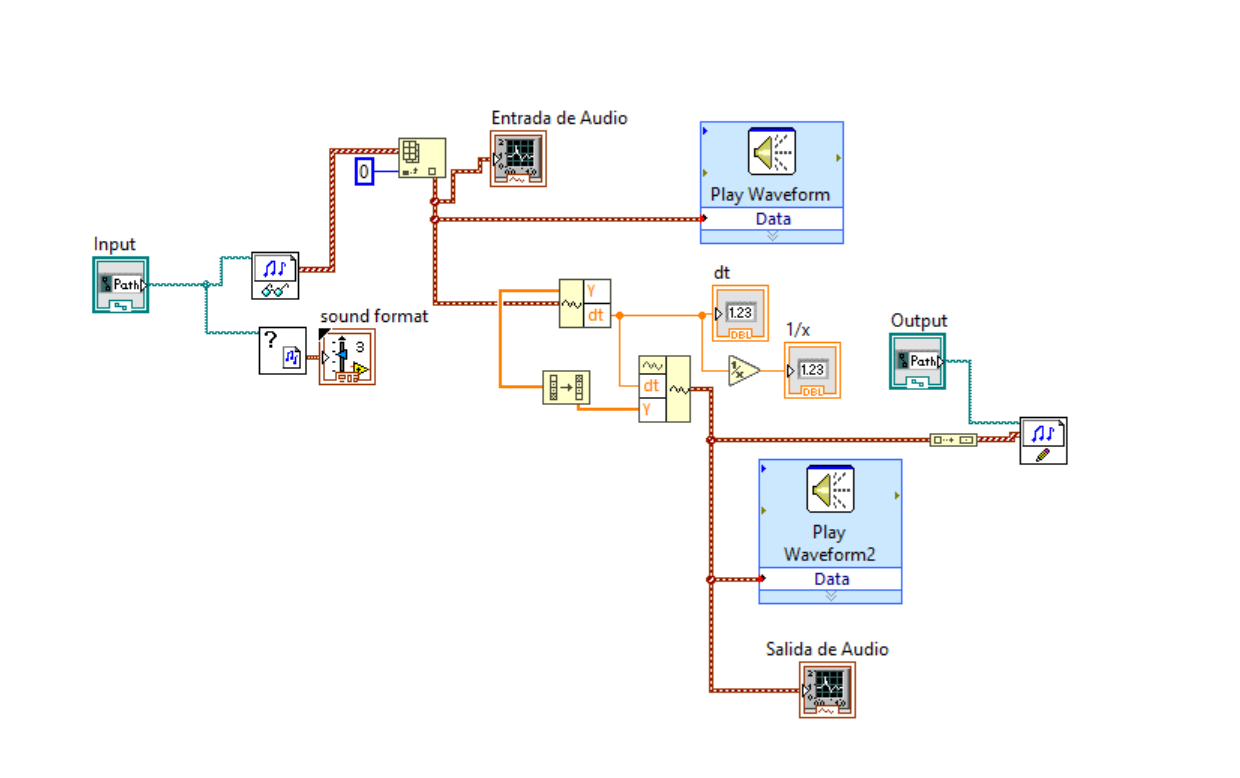
\includegraphics[width=\columnwidth]{images/11_labview_modelado.png}
\caption{Diagrama de bloques (VI) implementado en LabVIEW: lectura de audio, cálculo de $dt$ y $1/dt$, inversión del arreglo temporal y reproducción/almacenamiento de la señal de salida.}
\label{fig:labview_vi}
\end{figure}

La Figura \ref{fig:labview_invertido} compara un acercamiento al inicio de la señal de entrada (0 a 10~ms) con el correspondiente acercamiento al final de la señal de salida invertida (240 a 250~ms, extremo final de una señal de 250~ms). Se observa que la forma de onda de la entrada en sus primeras muestras coincide, en orden inverso, con la forma de onda de la salida en sus últimas muestras, confirmando que la inversión del arreglo temporal se ejecutó correctamente. Esta inversión conserva el contenido espectral de la señal, ya que la magnitud de la FFT de una señal real invertida en el tiempo es idéntica a la de la señal original; lo que se pierde es únicamente la información de orden temporal, relevante para el diseño de un decodificador secuencial que deba reconstruir la secuencia de dígitos marcados en su orden correcto.

\begin{figure}[!t]
\centering
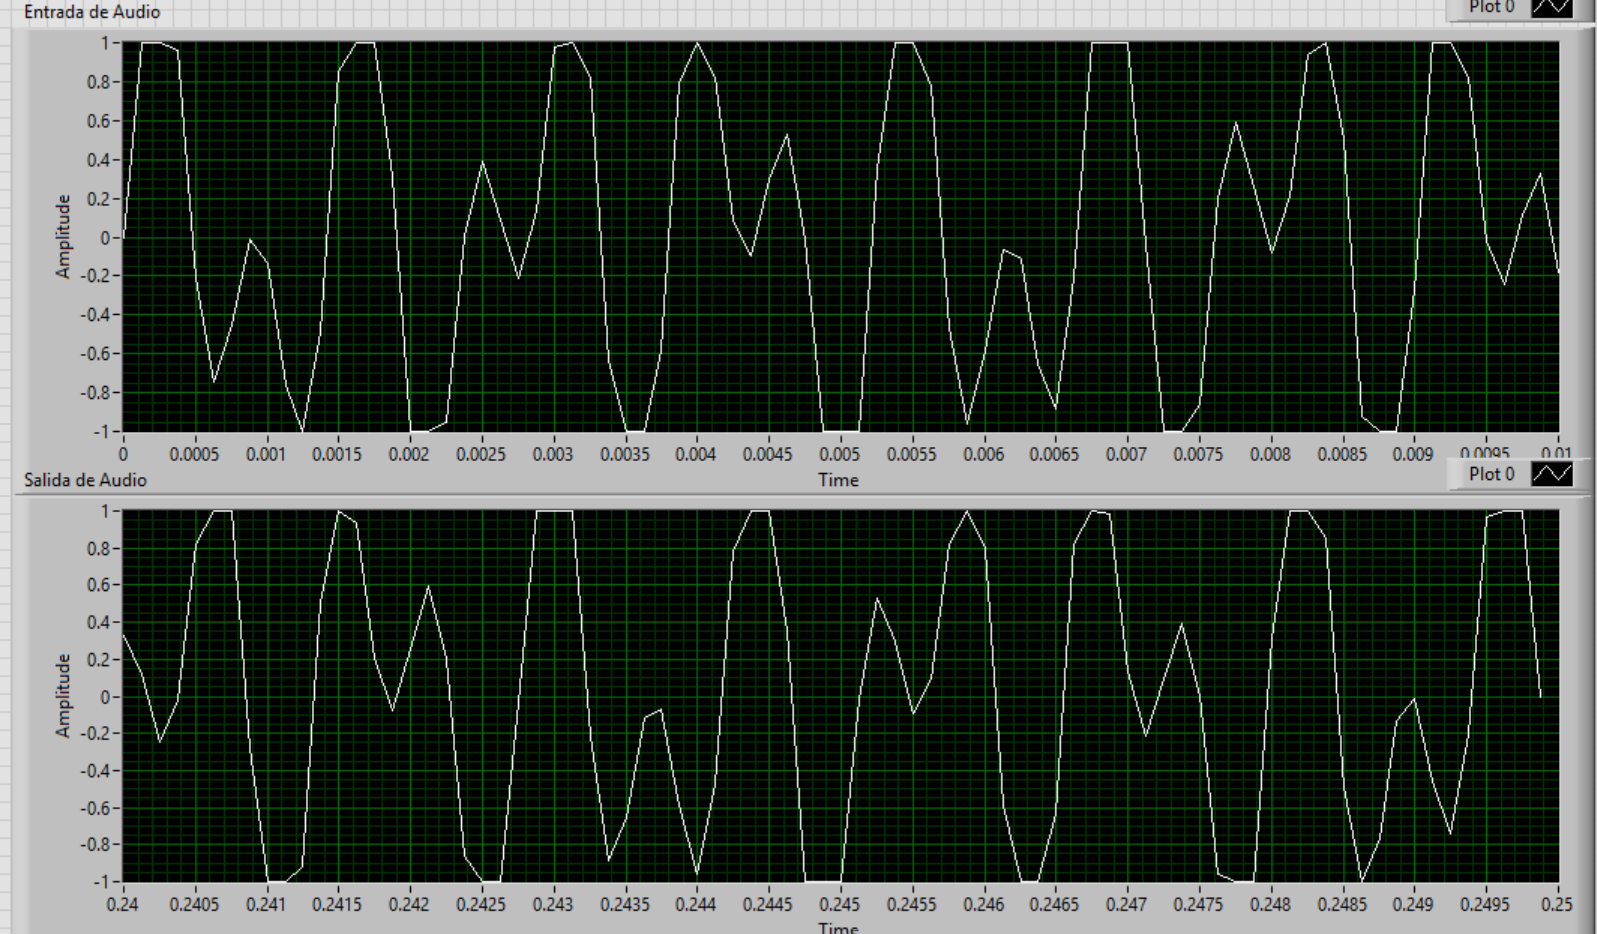
\includegraphics[width=\columnwidth]{images/13_labview_audio_invertido.png}
\caption{Comparación entre el inicio de la señal de entrada (arriba) y el final de la señal de salida invertida (abajo), evidenciando que el arreglo fue invertido en el tiempo conservando su contenido espectral.}
\label{fig:labview_invertido}
\end{figure}

\subsection{Modelo Simulink \texttt{dspdtmf}}

El modelo de referencia \texttt{dspdtmf} de la \textit{DSP System Toolbox} de MATLAB está organizado en bloques funcionales cuyo rol es el siguiente:

\begin{itemize}
    \item \textbf{Generator (Generador DTMF):} produce la secuencia de tonos DTMF a partir de los dígitos marcados, análogo a la etapa de generación implementada en la Sección IV-B mediante la ecuación \eqref{eq:dtmf_signal}.
    \item \textbf{Channel (Canal):} modela las imperfecciones del medio de transmisión, típicamente agregando ruido y/o atenuación, de forma análoga a las Secciones V-C y V-E de este informe.
    \item \textbf{Receiver (Receptor):} implementa el algoritmo de detección de tonos (habitualmente basado en el algoritmo de Goertzel) que estima las dos frecuencias presentes y decodifica el dígito correspondiente, cumpliendo el rol del decodificador automático descrito en la Sección IV-G.
    \item \textbf{Spectrum Analyzer:} visualiza el contenido espectral de la señal en tiempo real, permitiendo verificar visualmente la presencia y posición de los dos picos DTMF, de forma equivalente a las figuras de FFT presentadas en este informe.
    \item \textbf{Scope:} muestra la forma de onda en el dominio del tiempo, permitiendo verificar la superposición de tonos y silencios de la secuencia marcada.
\end{itemize}

El filtro pasa-banda (implícito en la etapa de \textit{Channel}/\textit{Receiver} de modelos DTMF más completos) es importante porque restringe la energía analizada a la banda de 600--1700~Hz donde residen las ocho frecuencias DTMF, atenuando ruido y componentes de voz fuera de banda antes de la etapa de detección, lo que mejora directamente el SNR efectivo visto por el algoritmo de detección de picos, de forma análoga a la restricción de rango aplicada en el decodificador de la Sección IV-G. El ancho de banda de este filtro incide directamente en la precisión y el desempeño de la detección: un filtro demasiado angosto puede atenuar o distorsionar el propio tono DTMF si su frecuencia central no coincide exactamente con la nominal (por ejemplo, por corrimiento Doppler o imprecisión del oscilador transmisor), mientras que un filtro demasiado ancho deja pasar más energía de ruido y de voz, degradando el SNR efectivo y aumentando la tasa de falsos positivos; el diseño típico busca un ancho de banda ligeramente mayor a la resolución espectral mínima requerida ($\Delta f = 1/T$ de la Sección III-C) pero lo suficientemente estrecho para rechazar las frecuencias DTMF vecinas y las componentes de voz.

Respecto a la comparación entre DFT y el algoritmo de Goertzel: la DFT (o su implementación eficiente, la FFT) calcula el espectro completo de la señal en todas las frecuencias del contenedor de resolución, con un costo computacional de $O(N \log N)$, siendo apropiada cuando se requiere observar el espectro completo, como se hizo en este informe. El algoritmo de Goertzel, en cambio, evalúa la magnitud espectral únicamente en un conjunto reducido de frecuencias predefinidas (las ocho frecuencias DTMF) con un costo de $O(N)$ por frecuencia evaluada, lo que resulta significativamente más eficiente en sistemas embebidos de detección DTMF en tiempo real, donde solo interesan esas ocho frecuencias y no el espectro completo \cite{proakis}.

En cuanto al uso de redes neuronales frente a métodos tradicionales (FFT/Goertzel) para la detección de tonos DTMF, los métodos tradicionales presentan la ventaja de ser deterministas, computacionalmente económicos y directamente interpretables en términos físicos (la posición de un pico espectral corresponde de forma directa a una frecuencia), por lo que continúan siendo el estándar de la industria para esta tarea bien definida y de bajo número de clases (dieciséis dígitos posibles). Una red neuronal podría, en principio, aprender a clasificar patrones espectro-temporales más robustos frente a ruido no gaussiano o distorsión no lineal del canal, pero introduce un costo computacional y de memoria mayor, requiere entrenamiento con datos representativos y pierde la garantía analítica de exactitud en frecuencia que ofrece Goertzel; por ello, su uso solo se justificaría en escenarios con fuentes de degradación complejas y no modelables analíticamente, y no en la detección DTMF convencional, donde el problema está completamente caracterizado por ecuaciones \eqref{eq:dtmf_signal}--\eqref{eq:atenuacion}.

Finalmente, para evaluar experimentalmente el desempeño de un receptor DTMF real bajo distintas condiciones de canal se propone el siguiente diseño experimental, coherente con la metodología ya aplicada en este informe: (1) generar un conjunto de prueba con los dieciséis dígitos DTMF, cada uno repetido un número suficiente de veces (por ejemplo, 100 repeticiones por dígito) para obtener significancia estadística; (2) para cada repetición, aplicar de forma independiente y combinada las tres condiciones de degradación estudiadas —ruido AWGN variando el SNR en pasos de 5~dB entre 30 y $-5$~dB, atenuación de línea variando entre 0 y $-30$~dB, y distorsión no lineal (por ejemplo, recorte o \textit{clipping} suave)— replicando así las condiciones de canal simuladas en las Secciones V-C y V-E; (3) ejecutar el receptor bajo prueba (basado en FFT, Goertzel, o el método que se desee evaluar) sobre cada señal degradada y registrar el dígito decodificado. Como métricas de evaluación se proponen: la tasa de detección correcta (porcentaje de dígitos correctamente decodificados), la tasa de falsos positivos (dígitos reportados en ausencia de tono válido o silencio erróneamente clasificado como dígito), la tasa de falsos negativos (tonos válidos no detectados), el error absoluto medio de la frecuencia estimada respecto a la teórica, y el SNR mínimo o la atenuación máxima para los cuales la tasa de detección correcta se mantiene por encima de un umbral de aceptación (por ejemplo, 99\%, valor típico exigido por las recomendaciones de señalización telefónica). Graficar estas métricas en función del nivel de degradación permite construir curvas de desempeño análogas a las curvas de tasa de error de bit (BER) usadas en sistemas de comunicaciones digitales, y así comparar objetivamente distintos algoritmos de detección bajo las mismas condiciones de canal.

\section{Conclusión}

Se generó, reprodujo y analizó exitosamente la señal DTMF correspondiente a la secuencia de marcación ``582A*'' mediante simulación en MATLAB, verificando en el dominio del tiempo la superposición de dos componentes sinusoidales por dígito y, en el dominio de la frecuencia, la presencia de dos picos espectrales dominantes coincidentes con la tabla DTMF estándar, con errores de detección de frecuencia de 0.260\% (componente baja) y 0.000\% (componente alta) para el dígito de referencia ``5''. El decodificador automático basado en FFT y detección de picos identificó correctamente el 100\% de los cinco dígitos de la secuencia de prueba.

El análisis de robustez mostró que el ruido AWGN constituye la condición más crítica para la detección: a SNR de 0~dB el piso espectral alcanza magnitudes comparables a las de los picos DTMF, mientras que a 10~dB o más la detección permanece viable. La reducción de la duración del tono degrada la resolución espectral según $\Delta f = 1/T$, ensanchando los picos y reduciendo el margen de tolerancia frente a otras fuentes de error, aunque en el rango evaluado (50--500~ms) no impidió la identificación de los tonos. La atenuación de línea, por su parte, escala uniformemente la amplitud de la señal sin alterar la posición de las frecuencias DTMF, por lo que su riesgo principal es indirecto, al reducir el margen de SNR disponible frente al ruido del canal.

El modelo complementario en Simulink, construido con bloques de fuente sinusoidal, suma, retenedor de orden cero y exportación a \textit{workspace}, reprodujo resultados consistentes con el análisis directo en MATLAB (errores de 0.210\% y 0.050\%), validando el enfoque de modelado por bloques para representar la cadena de generación y muestreo de una señal DTMF. Finalmente, la discusión conceptual sobre LabVIEW y el modelo Simulink \texttt{dspdtmf} permitió relacionar los resultados obtenidos con la arquitectura típica de un detector DTMF real, identificando el algoritmo de Goertzel y el filtrado pasa-banda como mejoras prácticas de eficiencia y robustez frente a la FFT completa utilizada en este informe.

\bibliographystyle{IEEEtran}
\bibliography{references}

\end{document}